
\chapter{Éléments de géométrie différentielle}

\section{Une première approche heuristique}
Nous développerons lors de ce chapitres les bases nécessaires pour étudier la géométrie d'un espace-temps courbe. Formellement, ceci nécessite d'une connaissance de topologie, et un lecteur intéressé est invité à se renseigner sur le sujet. Pour des raisons pégagogiques, nous allons omettre une définition mathématiquement rigoureuse (via les espaces topologiques de Hausdorff). \\
\\
L'étude d'un espace courbe pose problème : il ne s'agit plus d'un espace vectoriel. Ceci aura comme conséquence que la notion de vecteur perd sa caractéristique globale : nous ne pourrons plus comparer deux vecteurs qui se situent à des points lointains. Cette première section servira à introduire de manière heuristique (c'est-à-dire, avant de définir ce qu'est une variété différentielle). La deuxième section introduira cette notion à proprement dit et retouchera sur les notions de vecteurs. Nous consacrerons ensuite quelques pages pour discuter des p-formes différentielles.
\subsection{Espace tangent}
On se place encore dans l'espace-temps de Minkowski $\mathcal{M}= \R^{1,3}$ avant de généraliser les concepts à une variété différentielle arbitraire.

\begin{theoremframe}
    \begin{notat}
    Soit $P\in \mathcal{M}$. L'espace tangent à $\mathcal{M}$ au point $P$ est noté $T_P\mathcal{M}$. C'est un espace vectoriel réel de dimension 4.
    \end{notat}
\end{theoremframe}
La définition précise d'un espace tangent sera donné ultérieurement. Les éléments de $T_P\mathcal{M}$ sont appelés \textit{vecteurs} au point $P$. 
\begin{rmk}
La notion locale (au point $P$) de cette définition est importante: un vecteur ne pourra pas être vu comme une flèche rejoignant le point $P$ à un autre point $Q \in \mathcal{M}$. Le vecteur \textit{ne vit pas} sur le même espace que les points $P$ et $Q$. Lorsque $\mathcal{M} = \R^{1,3}$, il n'y a pas de problème car les ensembles $\mathcal{M}$ et $T_P\mathcal{M}$ coincident. On peut alors les voir comme des flèches rejoignant deux points distincts. Ceci n'est plus le cas si l'espace-temps est courbe.
\end{rmk}
\begin{theoremframe}
\begin{defi}
    L'union disjointe de tous les espaces tangents de $\mathcal{M}$ noté $T\mathcal{M}=\bigsqcup_P T_P\mathcal{M}$ est appelé \textit{fibré tangent} de $\mathcal{M}$.
\end{defi}
\end{theoremframe}
Comme $T_P\mathcal{M}$ est un espace vectoriel à 4 dimensions, il existe une base de vecteurs $\{\overline{e}_\alpha\}_\alpha$ de $T_P\mathcal{M}$ où $\alpha = \{0,1,2,3\}$. Un vecteur $V \in T_P\mathcal{M}$ peut donc être décomposé sur cette base selon $V = V^\alpha \overline{e}_\alpha$, où $V^\alpha$ sont les composantes du vecteur $V$. Remarquons donc que bien que $V$ ne dépend pas du choix de la base, $V^\alpha$, quant à lui, dépend bien de ce choix.

La donnée d'un vecteur $x_{P} \in T_{p}\mathcal{M}$ à tout $P$ de l'espace est un champ de vecteurs.

Un ensemble canonique de vecteur de $\mathcal{M}$ est un vecteur tangent à une courbe. 

\begin{theoremframe}
    \begin{defi}
        Soit une courbe lisse $\R \to \mathcal{M}: \lambda \mapsto x^\mu (\lambda)$. Le vecteur tangent à la courbe est
        \begin{equation}
            V^\alpha = \frac{\td x^\alpha}{\td \lambda}
        \end{equation}
    \end{defi}
\end{theoremframe}
\begin{theoremframe}
\begin{propri}
    Soit un vecteur $V^\alpha\in T_P\mathcal{M}$. Sous transformation de Poincaré, ce vecteur se transforme comme
    \begin{equation}
        V^{\alpha'} = \Lambda^{\alpha'}_{\; \mu} V^\mu
    \end{equation}
\end{propri}
\end{theoremframe}
\begin{proof}
    Soit une courbe lisse $x^\mu(\lambda)$. Sous transformation de Poincaré, cette courbe se transforme comme $x^{\mu'} = \Lambda^{\mu'}_{\; \mu} x^\mu + a^{\mu'}$. Notons $V^\mu$ le vecteur tangent à la courbe au point $P$. Alors, par définition de $V$, on trouve
    \begin{align}
        V^{\mu'} = \frac{\td x^{\mu'}}{\td \lambda} = \Lambda^{\mu'}_{\; \mu} \frac{\td x^{\mu}}{\td \lambda} = \Lambda^{\mu'}_{\; \mu} V^\mu
    \end{align}
\end{proof}
\begin{theoremframe}
    \begin{propri}
        Sous transformation de Poincaré, les vecteurs de base se transforment comme
        \begin{equation}
            \overline{e}_{\mu '} = \Lambda^{\cdot\,\mu}_{\mu'}\overline{e}_{\mu}
        \end{equation}
    \end{propri}
\end{theoremframe}
\begin{proof}
La décomposition d'un vecteur dans deux référentiels inertiels différents s'écrit
    \begin{equation}
    V = V^{\mu} \overline{e}_{\mu} = V^{\alpha '} \overline{e}_{\alpha '}
\end{equation}
Ainsi,
\begin{equation}
    V^{\alpha '} \overline{e}_{\alpha '} = \Lambda^{\alpha'}_{\; \mu} V^\mu \overline{e}_{\alpha '} = V^\mu \overline{e}_{\mu}
\end{equation}
Comme ceci est valable pour $V^\mu$ arbitraire, on conclut que 
\begin{equation}
    \Lambda^{\alpha'}_{\; \mu} \overline{e}_{\alpha '} = \overline{e}_{\mu}.
\end{equation}
En remarquant que $\Lambda$ vérifie
\begin{equation}
    \Lambda^\alpha_{\;\mu} \eta_{\alpha\beta} \Lambda^\beta_{\;\nu} = \eta_{\mu\nu}
\end{equation}
on trouve la propriété
\begin{equation}
    \label{eq:id lambda}
    \Lambda^\alpha_{\;\mu} \Lambda^{\cdot\,\nu}_\alpha = \delta^{\cdot\, \nu}_\mu
\end{equation}
où le point clarifie l'ordre des indices. Ceci permet de conclure, en multipliant par $\Lambda^{\cdot\,\nu}_\alpha$ que
\begin{equation}
    \overline{e}_{\alpha '} = \Lambda^{\cdot\,\mu}_{\alpha'}\overline{e}_{\mu}
\end{equation}
\end{proof}

\subsection{Espace co-tangent}
\begin{theoremframe}
    \begin{defi}
        Une forme linéaire sur un espace vectoriel $(\mathcal{V},\mathbb{K})$ est une application linéaire $w:\mathcal{V} \to \mathbb{K}$. Pour $a,b\in \mathbb{K}$ et $X,Y \in \mathcal{V}$, on a donc
        \begin{equation}
            w(aX+bY) = aw(X)+bw(y)
        \end{equation}
    \end{defi}
\end{theoremframe}
Nous appelons \textit{dual} d'un espace vectoriel $V$ l'ensemble des formes linéaires sur cet espace.
\begin{theoremframe}
    \begin{defi}
        L'espace \textit{co-tangent} à $\mathcal{M}$ en un point $P$ est le dual de $T_P\mathcal{M}$ et est noté $T_P^*\mathcal{M} = (T_P\mathcal{M)^*}$.
    \end{defi}
\end{theoremframe}
\begin{theoremframe}
    \begin{defi}
        Un \textit{covecteur} est un élément de l'espace co-tangent $w\in T_P^*\mathcal{M}$.
    \end{defi}
\end{theoremframe}
On peut définir une base $\{\Theta^\mu\}_\mu$ sur l'espace co-tangent selon l'identité
\begin{equation}
    \Theta^\mu(\overline{e}_\nu)=\delta^\mu_\nu
\end{equation}
Dans cette base, un covecteur $w\in T_P^*\mathcal{M}$ s'écrit $w = w_\alpha \theta^\alpha$. Soit $V \in T_P\mathcal{M}$:
\begin{align}
    w(V) &= w_{\alpha} \Theta^{\alpha}(V^{\mu} \Vec{e_{\mu}})\\
    &=w_{\alpha} V^{\mu}\Theta^{\alpha} (\Vec{e_{\mu})}\\
    &= w_{\alpha} V^{\mu}\delta^{\alpha}_{\mu}\\
    &= w_{\alpha} V^{\alpha} \in \R
\end{align}


où $V$ est un vecteur de l'espace tangent. 

Cette expression ne dépend pas du choix de base. De plus, elle ne comporte pas d'indices libres. Un tel terme est appelé scalaire de Lorentz. On peut l'écrire de manière équivalente comme $w(V) = w_{\alpha} V^{\alpha} = w_{\alpha '} V^{\alpha '} $.
\begin{rmk}
    Dans un espace vectoriel de dimension finie, le dual de l'espace dual est identifié à $T_P\mathcal{M}$. On a donc $(T^*_P\mathcal{M})^* = T_P\mathcal{M}$.
\end{rmk} 
\begin{theoremframe}
    \begin{propri}
        Soit un covecteur $V^\alpha\in T^*_P\mathcal{M}$. Sous transformation de Poincaré, ce covecteur se transforme comme
    \begin{align}
        w_{\alpha'} = \Lambda^{\cdot \, \mu}_{\alpha'} V^\mu
    \end{align}
    \end{propri}
\end{theoremframe}
\begin{proof}
    On vient de voir que $w(V)$ est un scalaire de Lorentz:
    \begin{equation}
        w(V) = w_{\alpha} V^{\alpha} = w_{\alpha '} V^{\alpha '} 
    \end{equation}
    Et donc par la loi de transformation d'un vecteur, on a
    \begin{equation}
        w_{\alpha} V^{\alpha} = w_{\alpha '} \Lambda^{\alpha '}_{\;\mu} V^\mu
    \end{equation}
    Comme ceci est valable pour tout vecteur $V$, on peut écrire
    \begin{equation}
        w_{\alpha}  = w_{\alpha '} \Lambda^{\alpha '}_{\;\alpha}
    \end{equation}
    Et on trouve le résultat recherché en utilisant l'identité \ref{eq:id lambda}.
\end{proof}

En particulier, la base de l'espace co-tangent se transforme comme:
$$ \Theta^{\alpha '} = \Lambda^{\alpha '}_{\; \mu} \Theta^{\mu}$$

\begin{theoremframe}
    \begin{defi}
        L'union de tous les espaces co-tangents de $\mathcal{M}$ noté $\bigcup_P T^*_P\mathcal{M}$ est appelé \textit{fibré co-tangent} de $\mathcal{M}$.
    \end{defi}
\end{theoremframe}
Maintenant qu'on a explicité l'emplacement des indices corrects, nous n'allons plus l'indiquer pour le reste de ce syllabus afin de simplifier les notations.

\subsection{Les tenseurs}

On peut généraliser les notions de vecteur et covecteur à un tenseur. Si on considère un vecteur $V \in T_{p}\mathcal{M} : T^*_{p}\mathcal{M} \rightarrow \mathbb{R}$ et un covecteur $w \in T^*_{p}\mathcal{M} : T_{p}\mathcal{M} \rightarrow \mathbb{R}$, alors on peut voir le vecteur $V$ comme un tenseur $(1, 0)$ et on peut voir le covecteur $w$ comme un tenseur $(0, 1)$. 
\begin{theoremframe}
    \begin{defi}
        Un tenseur de type $(k, l)$ au point $P$ est une application multilinéaire
        \begin{equation}
            \underbrace{T^*_{p}\mathcal{M} \times \cdots \times T^*_{p}\mathcal{M}}_\text{$k$-fois} \times \underbrace{T_{p}\mathcal{M} \times \cdots \times T_{p}\mathcal{M}}_\text{$l$-fois}  \to \mathbb{R}
        \end{equation}

        Multilinéaire signifie linéarité en chaque variable, donc par exemple pour un tenseur de type $(1,1)$: 
        \begin{equation}
        T(aw +b\eta, cX +dY) = acT(w, X) + adT(w, Y) + bcT(\eta, X) +cdT(\eta, Y)
        \end{equation}
        où $a,b, c ,d \in \mathbb{R}$
    \end{defi}
\end{theoremframe}
\begin{exmp}
    Un tenseur $(1, 1)$ est tel que $T(w,V) \in \R$ où $w$ est un covecteur et $V$ est un vecteur. 
\end{exmp}
\begin{exmp}
    Si un tenseur $T$ est tel que pour $V\in T_p\mathcal{M}$, on a $T(V) \in T^*_p\mathcal{M}$, alors il s'agit d'un tenseur de type (0,2).
\end{exmp}
\begin{theoremframe}
    \begin{propri}
        L'ensemble des tenseurs de type $(k, l)$ en $P\in \mathcal{M}$ forment un espace vectoriel. Une base de cette espace vectoriel est donnée par 
        \begin{equation}
        \overline{e}_{\alpha_1} \otimes \cdots \otimes \overline{e}_{\alpha_k} \otimes \Theta^{\mu _1}\otimes \cdots \otimes \Theta^{\mu _l}
        \end{equation}
    \end{propri}
\end{theoremframe}
Un tenseur de type $(k,l)$ se décompose donc sur cette base comme
\begin{equation}
    T = T\indices{^{\alpha _1 \cdots \alpha _k}_{v_1 \cdots v_l}}\overline{e}_{\alpha_1} \otimes \cdots \otimes \overline{e}_{\alpha_k} \otimes \Theta^{v _1}\otimes \cdots \otimes \Theta^{v _l}
\end{equation}
\begin{theoremframe}
    \begin{propri}
        Un vecteur de type $(k,l)$ se transforme sous transformation de Poincaré comme\footnote{Ici, $\times$ est utilisé pour la multiplication usuelle et non comme produit direct.}
        \begin{equation}
            T\indices{^{\alpha ' _1 \cdots \alpha ' _k}_{v'_1 \cdots v'_l}} = \Lambda\indices{^{\alpha '_1}_{\alpha _1 }} \times \cdots \times \Lambda\indices{^{\alpha '_k}_{\alpha _k}} \times \Lambda\indices{_{v'_1 }^{v_1 }} \times \cdots \times \Lambda\indices{_{v'_k}^{v_k}} \times T\indices{^{\alpha _1 \cdots \alpha _k}_{v_1 \cdots v_l}}.
        \end{equation}
        La transformation implique donc $k+l$ matrices de Lorentz.
    \end{propri}
\end{theoremframe}
\begin{proof}
    Conséquence des propriétés précédentes.
\end{proof}

Revenons à la métrique de Minkowski. Celle-ci peut-être vue comme un tenseur $(2.0)$ symétrique.
\begin{equation*}
    \eta_{\mu ' \nu '} = \Lambda\indices{_{\mu '}^{\alpha}}\Lambda\indices{_{\nu ' }^{\beta}}\eta_{\alpha \beta}
\end{equation*}
De plus, la métrique de Minkowski est un invariant de Lorentz. Donc elle a les mêmes coordonnées dans tout référentiel inertiel.

\begin{theoremframe}
    \begin{defi}
        La métrique de Minkowski est un pseudo-produit scalaire pour l'espace $T_p\mathcal{M}$. En effet, celle-ci est une forme linéaire 
        \begin{align}
        \eta:\begin{pmatrix}
             T_p\mathcal{M} \times T_p\mathcal{M} & \to & \R\\
            (X,Y) & \mapsto & \eta(X,Y) = \eta_{\mu  \nu }X^{\mu}Y^{\nu}
        \end{pmatrix}
        \end{align}.
        En particulier, $\eta$ est symétrique et biliéaire.
    \end{defi}
    
\end{theoremframe}
\begin{rmk}
    Elle définit un pseudo-produit scalaire car elle n'est ni définie positive $\eta(X,X) \ngeq 0$, ni sépare les points $\eta(X,X) = 0 \centernot \implies X = 0$.
\end{rmk}
On dira que deux vecteurs sont orthogonaux si et seulement si $\eta (X, Y) = 0$. On note la norme d'un vecteur

\begin{align*}
    \lVert V \rVert ^2 = \eta (V, V) = \left\{
\begin{array}{l}
  < 0 \text{ si } V \text{est de genre temps} \\
  > 0 \text{ si } V \text{est de genre espace}\\
  = 0 \text{ si } V \text{est de genre lumière}
\end{array}
\right.
\end{align*}

La métrique permet d'établir un isomorphisme entre $T_{p}\mathcal{M} $ et $T^*_{p}\mathcal{M}$. C'est-à-dire qu'il permet d'associer un vecteur à un covecteur tel que

\begin{align*}
    \eta : \begin{pmatrix}
        T_{p}\mathcal{M} &\to & T^*_{p}\mathcal{M}\\
             V &\mapsto &\eta (V, \cdot)
    \end{pmatrix}
\end{align*}
Ceci justifie la convention que $\eta$ permet de monter ou descendre les indices tel que:

\begin{equation*}
    V^{\mu} \rightarrow \eta_{\mu \nu}V^{\mu} \equiv V_{\nu}
\end{equation*}

Donc par définition, l'espace temps de Minkowski est l'espace temps plat muni de la métrique de Minkowski. 

\subsection{Avantage de la notation tensorielle}
Outre le fait que la notation tensorielle permet une formulation plus compacte, on a également le résultat suivant:
\begin{theoremframe}
    \begin{prop}
        Si une relation tensorielle est valable dans un référentiel interiel alors elle sera valable dans tout référentiel inertiel.
    \end{prop}
\end{theoremframe}

Illustrons cette propriété avec les équations de Maxwell. Les équations de Maxwell sont des invariants de Lorentz mais c'est compliqué de le montrer explicitement (surtout pour les boosts). Une manière plus simple de le montrer est de les écrire en notation tensorielle, dans lesquelles elles seront nécessairement invariantes.

Les équations de Maxwell sont:

$$\left\{
\begin{array}{l}
  \vect{\nabla} \times \vect{B} -\partial_{t} \vect{E} = \vect{J}  \\
  \vect{\nabla} \cdot \vect{E} = \rho\\
  \vect{\nabla} \cdot \vect{B} = 0\\
  \vect{\nabla} \times \partial_t \vect{B} = \vect{0}
\end{array}
\right.$$

Pour écrire ces équations de manière tensorielle, on va définir le tenseur de Faraday (le tenseur de Faraday dépend du signe de la métrique ):


\begin{align}
\label{eq: Faraday}
 F_{\mu \nu}^{(-+++)} =  \begin{pmatrix}
0 & -E_1 & -E_2 & -E_3\\
E_1 & 0 & B_3 & -B_2\\
E_2 & -B_3 & 0 & B_1\\
E_3 & B_2 & -B_1 & 0\\
\end{pmatrix}   
\end{align}

Ce tenseur est antisymétrique $F_{\mu \nu}^{(-+++)} = - F_{\nu \mu}^{(-+++)}$

On peut réécrire les équations de Maxwell comme:

$$\left\{
\begin{array}{l}
  \partial_{\mu} F^{\mu \nu} = J^{\nu}(x) \\
  \partial_{[{\alpha}}F_{\mu \nu]} = 0(t)
\end{array}
\right.$$

où $J^{\mu} = (\rho, \Vec{J})$ est le quadri-courant.

La notation entre crochet est appelée anti-symétrisation et est défini par

\begin{equation}
    T_{[\mu_{1}, ... , \mu_{n}]} =\frac{1}{n!}(T_{\mu_{1}, ... , \mu_{n}} + \text{permutations signées des n indices})
\end{equation}

qui possède posséde $n!$ termes. 

\begin{exmp}
    \begin{equation*}
        T_{[\alpha \beta]} = \frac{1}{2!}\left(T_{\alpha\beta} - T_{ \beta \alpha}\right)
    \end{equation*}
\end{exmp}


On va montrer que la loi de Gauss peut s'écrire manière tensorielle.
On sait que la loi de Gauss est:

\begin{equation}
    \Vec{\nabla}\cdot \Vec{E} = \rho
\end{equation}
soit
\begin{equation}
    \partial_{i}E^{i} = J^{0}
    \label{loi de Gauss}
\end{equation}
\begin{rmk}
     On peut monter et descendre les indices spatiales sans conséquences $E^{i} = \eta^{ij}E_{j} = E_{i}$.
\end{rmk}

Par définition du tenseur de Faraday, on a
\begin{equation}
    F_{0i} = -E_i \text{ car } F_{01} = -E_1
\end{equation}
Remarquons que alors

\begin{equation}
    F^{0i} = \eta ^{0 \alpha} \eta ^{i\beta} F_{\alpha \beta} = (-)(+1)F_{0i} = -F_{0i} = E_j
    \label{Faraday}
\end{equation}

Donc en remplaçant le résultat \ref{Faraday} dans l'équation \ref{loi de Gauss}, on obtient:

\begin{equation}
    \partial_{i}F^{0i} = J^0
    \label{Loi de Gauss tensoirel}
\end{equation}

Comme $F^{\mu \nu}$ est antisymétrique, on a que $F^{00} = 0$. Donc on peut réécrire \ref{Loi de Gauss tensoirel} comme,

\begin{equation}
    \partial_{\alpha}F^{0\alpha} = J^0
\end{equation}

De manière similaire, il est possible d'intégrer la loi d'Ampère pour donner

\begin{equation}
    \label{eq:faraday tot}
    \partial_{\mu}F^{\mu\nu} = J^{\nu}
\end{equation}

Montrons que cette expression ne dépend effectivement pas du référentiel inertiel choisi. On sait que $x'^{\mu} = \Lambda^{\mu'}_{\alpha}x^{\alpha}$.
Donc on a que \ref{eq:faraday tot} peut se réécrire comme:

\begin{equation}
   \Lambda^{\nu '}_{\mu} \partial_{\nu '}(\Lambda ^{\mu}_{\alpha'}\Lambda ^{\nu}_{\beta '}F^{\alpha ' \beta '} ) =  \Lambda^{\nu }_{\alpha'}J^{\alpha '}
\end{equation}
par la loi de transformation tensorielle. Comme les matrices $\Lambda ^{\mu}_{\alpha'}$ et $\Lambda ^{\nu}_{\beta '}$ sont constantes, on peut les sortir de la dérivée. 

\begin{align}
   \overbrace{\Lambda^{\nu '}_{\mu} \Lambda ^{\mu}_{\alpha'}}^{\displaystyle\delta^{\nu '}_{\alpha' }}\Lambda ^{\nu}_{\beta '} \partial_{\nu '} F^{\alpha ' \beta '} & =  \Lambda^{\nu }_{\alpha'}J^{\alpha '} \\
   \implies \Lambda ^{\nu}_{\beta '} \partial_{\nu '} F^{\nu ' \beta '}  &=  \Lambda^{\nu }_{\alpha'}J^{\alpha '}
\end{align}

Et en multipliant des deux côtés par $\displaystyle\Lambda^\gamma_\nu$, on obtient bien

\begin{equation}
    \partial_{\alpha '}F^{\alpha ' \gamma '} = J^{\gamma '}
\end{equation}

Ceci montre bien que dans l'exemple des lois de Maxwell, l'expression tensorielle dans un système inertiel est en fait valable pour tout référentiel.

\section{Variétés différentielles}
Nous allons à présent considérer un espace-temps $\mathcal{M}$ avec courbure. Pour ce, il est utile d'introduire la notion de variété différentielle. Avant de voir celle-ci, nous rappellerons quelques notions de topologie.
\begin{theoremframe}
    \begin{defi}
        Soit $X$, un ensemble non-vide. Une collection $\mathcal{T}_X$ de sous-ensembles de $X$ est une \textit{topologie sur $X$} si
        \begin{itemize}
            \item[(i).] $X,\empty \in \mathcal{T}_X$.
            \item[(ii).] Si $U_1,\cdots,U_k \in \mathcal{T}_X$, alors $U_1 \cap \cdots \cap U_k \in \mathcal{T}_X$.
            \item[(iii).] Si $\{ U_i\}_{i\in I}$ est une collection quelconque d'éléments de $\mathcal{T}_X$, alors $\bigcup_{i\in I} U_i \in \mathcal{T}_X$.
        \end{itemize}
        Le couple $(X,\mathcal{T}_X)$ est un \textit{espace topologique}. Les éléments de $U\in \mathcal{T}_X$ sont les ouverts de l'espace topologique.
    \end{defi}
\end{theoremframe}
Sur base de cette définition, il est possible de reconstruire les notions d'analyse comme la continuité et la différentiabilité comme approche alternative à la notion séquentielle (via des suites). Nous n'allons pas aller en détail dans cette approche et directement passer au sujet de la géométrie différentielle.
\begin{theoremframe}
    \begin{defi}
        Une application sur des ouverts $f:U\to V$ est un \emph{homéomorphisme} si $f:U\to V$ est bijective et $f,f^{-1}$ sont continues. 
    \end{defi}
\end{theoremframe}
Notons que nous considérerons dans la suite que l'homéomorphisme sera lisse (c'est-à-dire $C^\infty$). L'utilité d'un homéomorphisme réside dans le fait qu'il préserve la structure topologique des espaces. Par exemple, Une tasse de café et un donut sont homéomorphes, car l'un peut être transformé en l'autre continûment, sans coupures.
\begin{theoremframe}
    \begin{defi}
        Un \textit{atlas} (lisse) d'un espace topologique $\mathcal{M}$ est une collection de paires $(U_i,\varphi_i) \quad {i\in I}$ telle que :
        \begin{itemize}
            \item[(i).] $\forall i\in I$, $U_i \in \mathcal{T}_\mathcal{M}$ et de plus, $\bigcup_{i\in I} U_i = \mathcal{M}$.
            \item[(ii).] $\varphi_i:U_i\to V_i$ où $V_i$ est un ouvert de $\R^m$ est un homéomorphisme.
            \item[(iii).] Si $U_i \cap U_j \neq \varnothing$, l'application 
            \begin{align}
            \varphi_{ij} = \varphi_i \circ \varphi^{-1}_j:\varphi_j(U_i\cap U_j) \subset \R^m \to \varphi_i(U_i\cap U_j) \subset \R^m 
            \end{align}
            est lisse. Cette fonction est également appelée la fonction de transition.
        \end{itemize}
    \end{defi}
\end{theoremframe}
\begin{theoremframe}
    \begin{defi}
        Une variété différentielle $\mathcal{M}$ de dimension $m$ est un espace topologique muni d'un atlas.
    \end{defi}
\end{theoremframe}
\begin{rmk} 
    \begin{enumerate}
        \item[\,] 
        \item L'application $\varphi_i^{-1}$ est appelée \emph{paramétrisation locale} de $\mathcal{M}$ sur $U_i\in \mathcal{M}$. Elle permet d'associer des coordonnées de $\R^m$ à chaque point de $U_i$. On dira que $\mathcal{M}$ ressemble localement à des ouverts de $\R^m$.
        \begin{figure}[H]
            \centering
            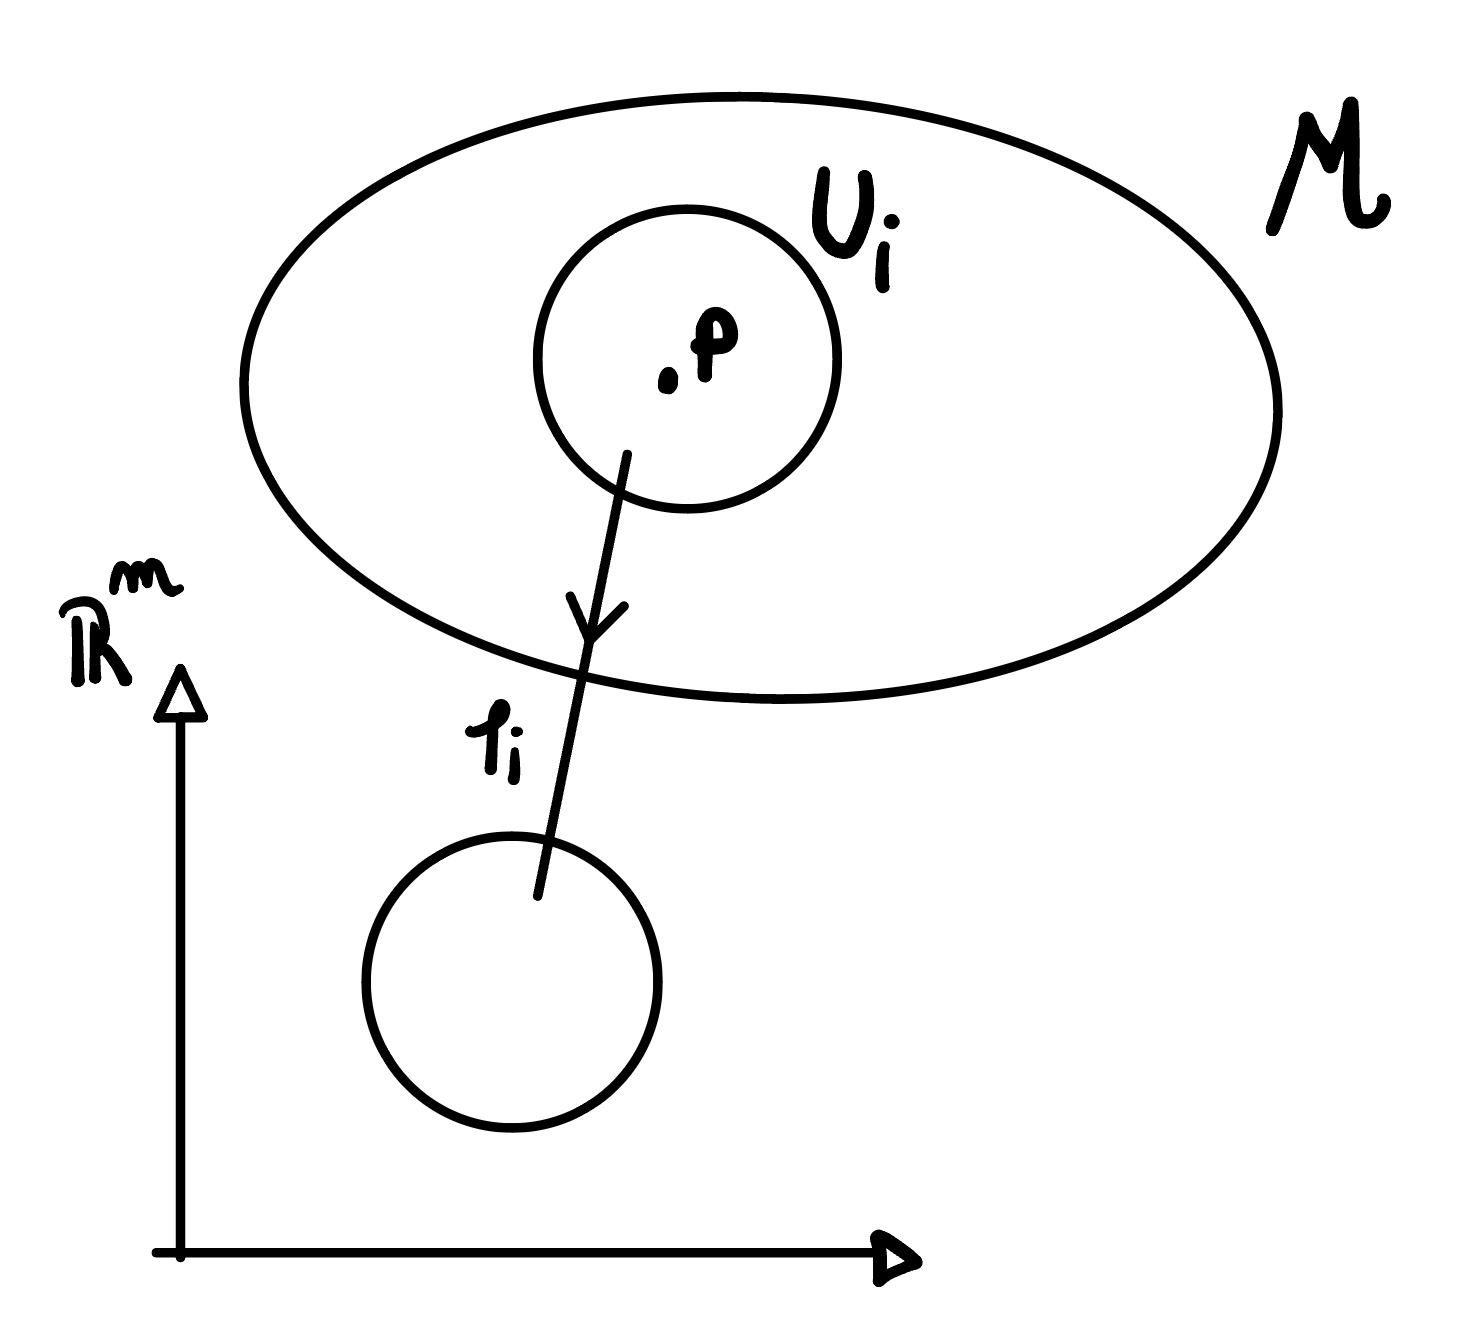
\includegraphics[width=0.3\linewidth]{Chapitres/3.Element de géométrie différentielle/Images/variété.jpg}
            \caption{}
            \label{fig:3.1}
        \end{figure}
        \item La condition (iii). impose que ces morceaux de $\R^m$ peuvent être "recollés" de manière lisse.
        \begin{figure}[H]
            \centering
            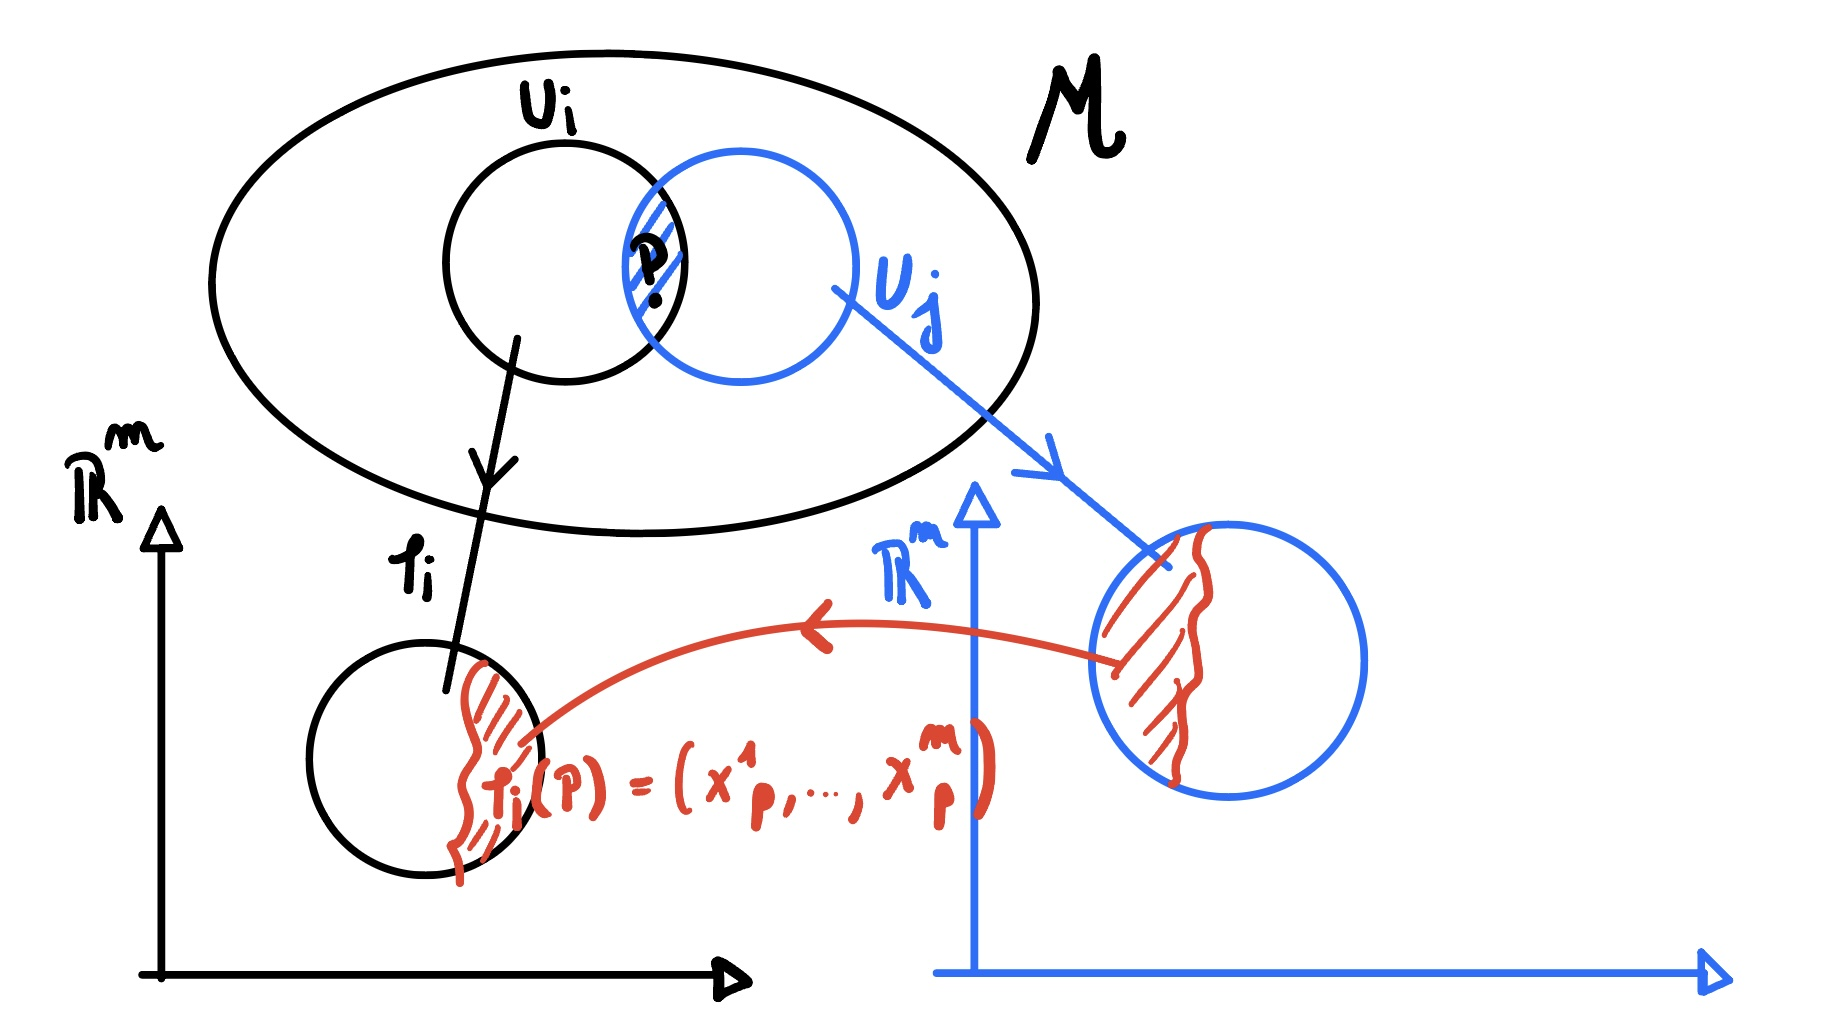
\includegraphics[width=0.5\linewidth]{Chapitres/3.Element de géométrie différentielle/Images/ouvertchevauchement.jpg}
            \caption{Sur les images de l'intersection de $U_i$ et $U_j$, il existe une bijection lisse.}
            \label{fig:3.2}
        \end{figure}
        \item Les atlas sur les variétés ne sont pas uniques. Les différents choix d'atlas correspond aux différents choix physique de système de coordonnées. La liberté de changer d'atlas correspond à la liberté de changer de coordonnées ou de référentiel pour décrire une variété.
    \end{enumerate}
\end{rmk}
    \begin{exerc}
        Montrez qu'un cône n'est pas une variété lisse. Pour rappel, le cône est défini comme 
        \begin{equation}
            C = \ltc (x,y,z)\in \R^3 \mid x^2+y^2-z^2=0, z\geq 0 \rtc
        \end{equation}
    \end{exerc}
\subsection{Application entre variété}
Soient deux variétés différentielles $\mathcal{M}$ et $ \mathcal{N}$ respectivement à cartes locales $(U,\varphi)$ et $(V,\psi)$ et une application continue $f:\mathcal{M} \to \mathcal{N}$.

\begin{theoremframe}
    \begin{defi}
        L'application $f$ est dite \emph{lisse} si et seulement si l'application 
        \begin{equation}
        F = \psi \circ f \circ \varphi^{-1}:\varphi(U) \to \psi(V)
        \end{equation}
        est lisse. Cette fonction est appelée \emph{représentation de coordonnées locales de} $f$.
    \end{defi}
\end{theoremframe}

\begin{center}
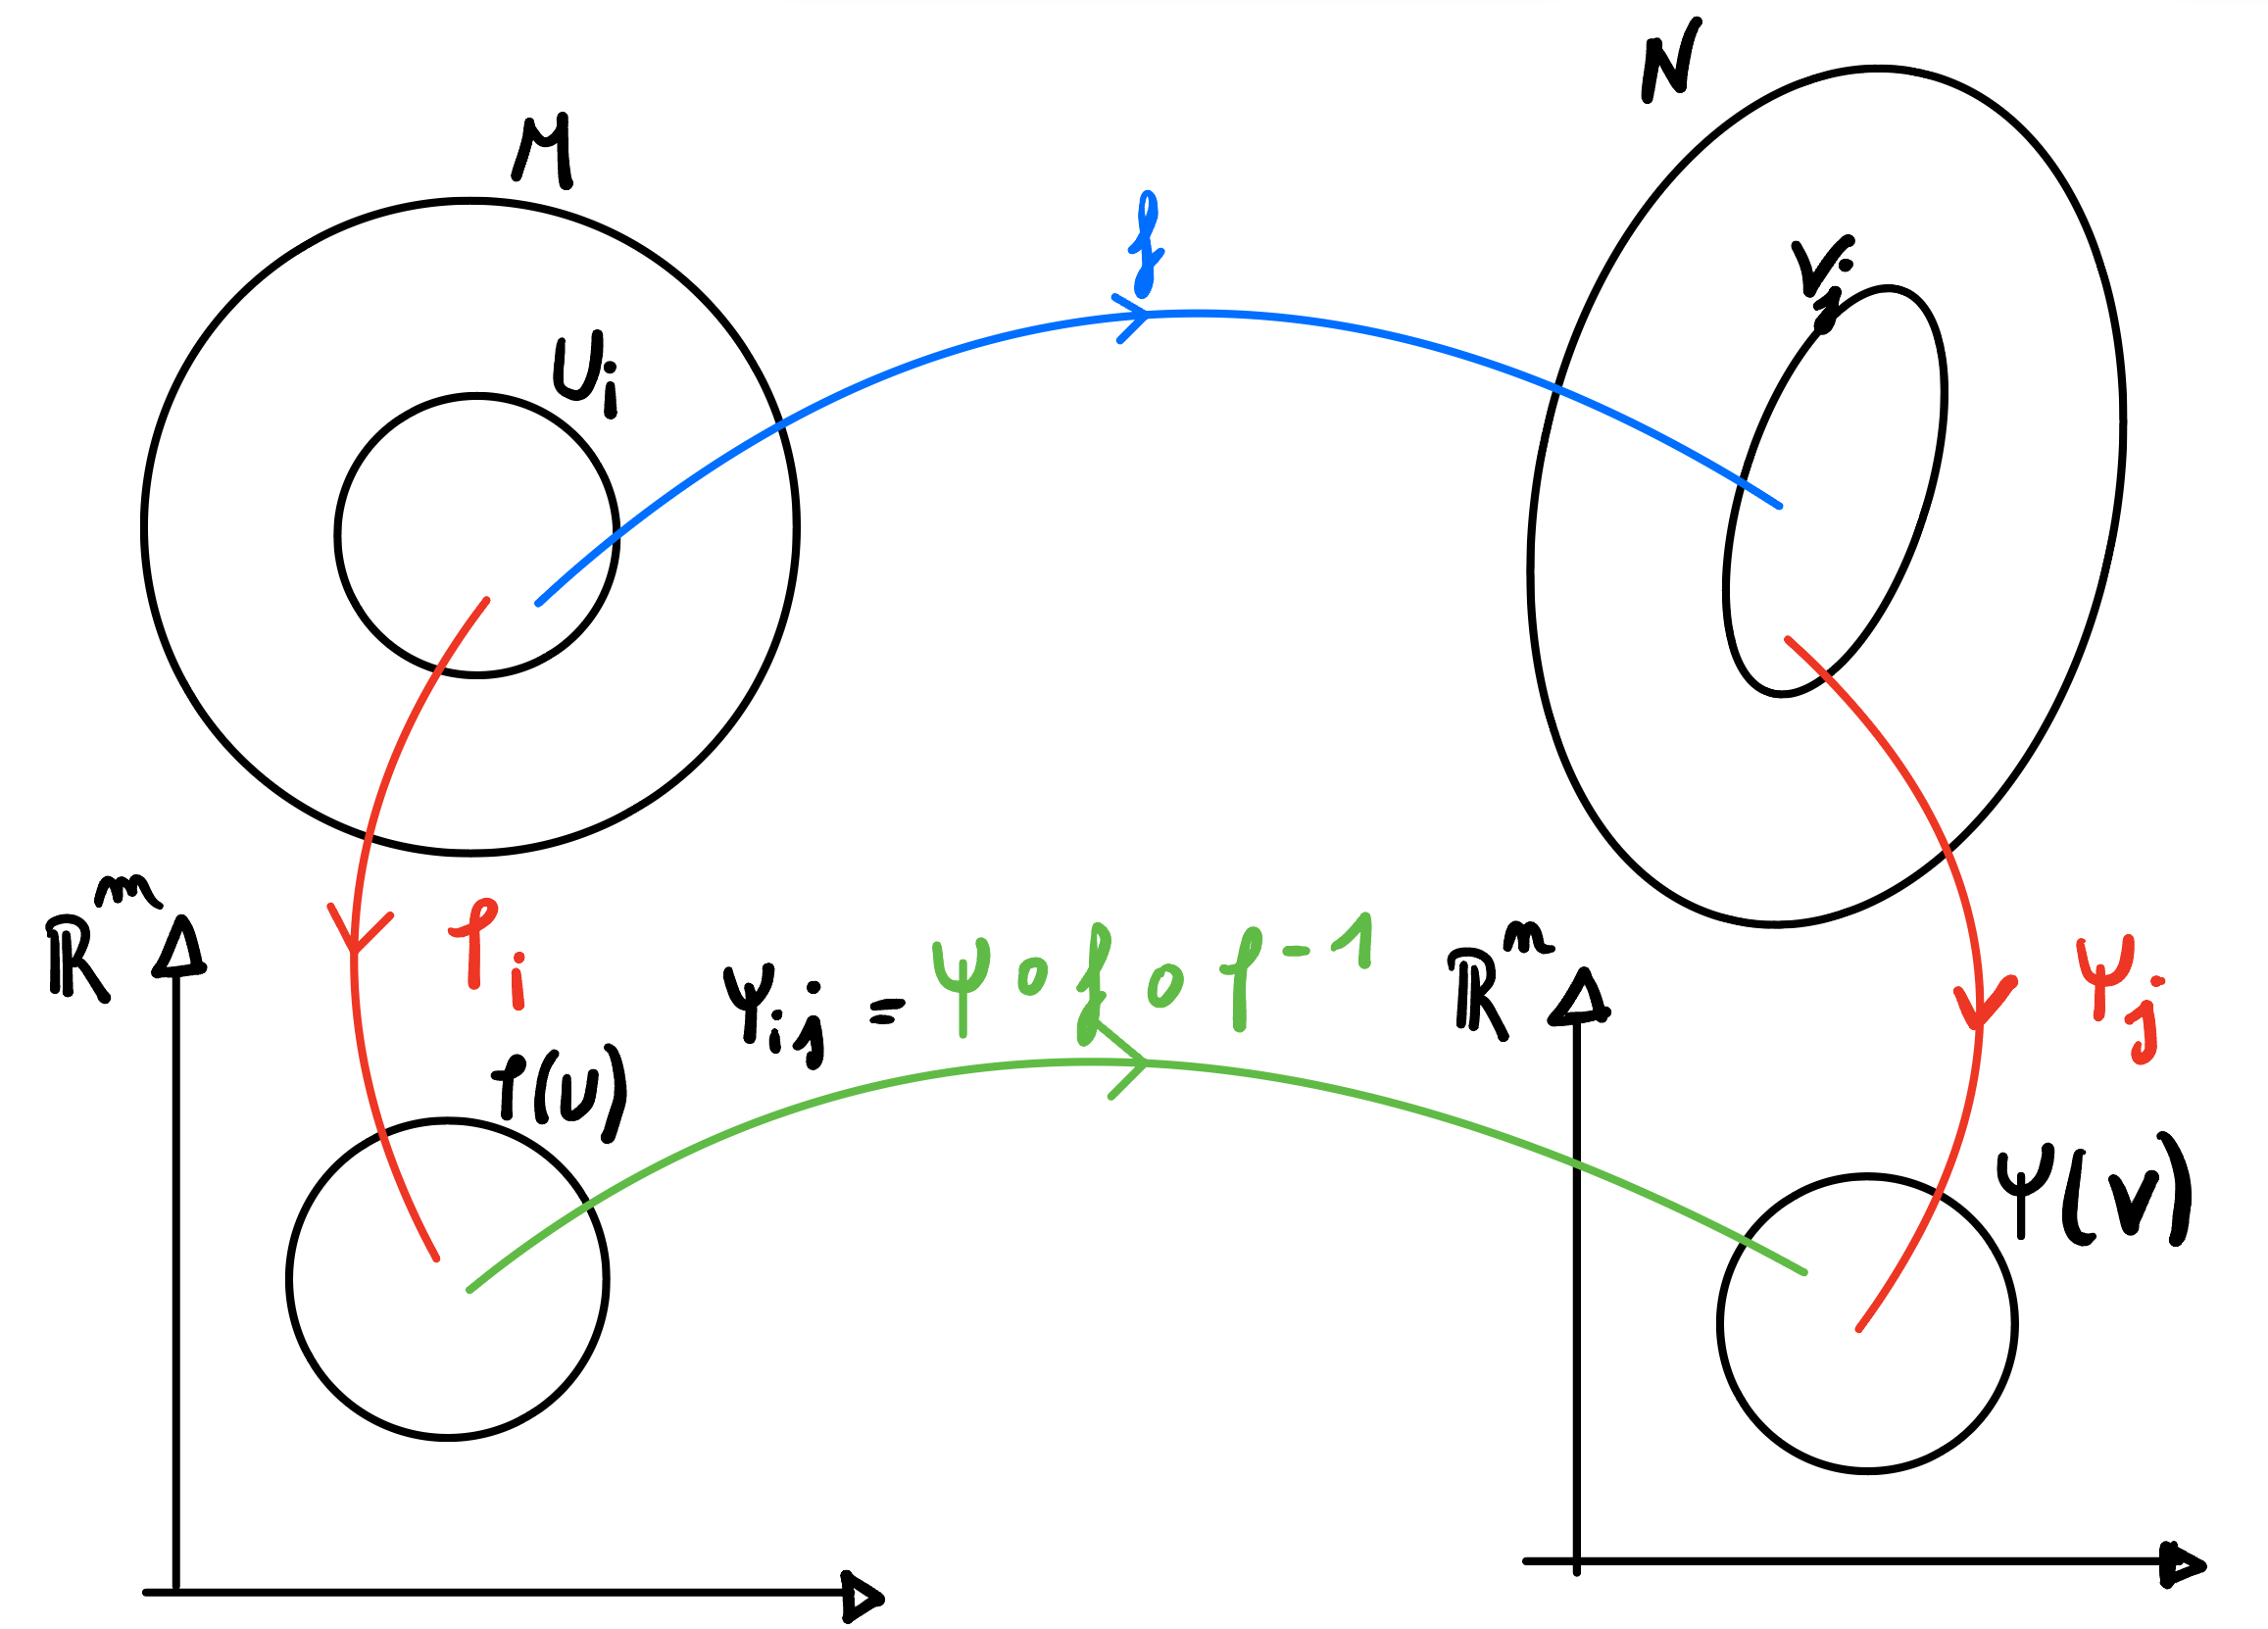
\includegraphics[scale=0.1]{Chapitres/3.Element de géométrie différentielle/Images/fonction de transistion.jpg}
%\captionof{figure}{}
%\label{Parabolique 2}
\end{center}

\subsection{Définition différomorphisme:}

Soient $\mathcal{M}$ et $\mathcal{N}$ deux variétés différentielle. 

\begin{theoremframe}
    \begin{defi}
        Une application $f:\mathcal{M} \to \mathcal{N}$ est un \emph{difféomorphisme} si et seulement si $f$ est bijective et si $f$ et $f^{-1}$ sont lisses. 
    \end{defi}
\end{theoremframe}
Alternativement, $f$ est un difféomorphisme si et seulement si il existe une application lisse $g: \mathcal{N} \to \mathcal{M}$ telle que 
\begin{equation}
    f \circ g = \mathrm{Id}_\mathcal{N} \quad \text{et} \quad g \circ f = \mathrm{Id}_\mathcal{M}
\end{equation}
Lorsqu'il existe un difféomorphisme entre $\mathcal{M}$ et $\mathcal{N}$, on dit qu'ils sont difféomorphes. Deux variétés qui sont difféomorphes sont également dites équivalent. On peut les déformer l'un dans l'autre de manière lisse. Un difféomorphisme va, contrairement à l'homéomorphisme non-lisse, préserver la structure différentielle et non-seulement la structure topologique de la variété. Ainsi, un cube est homéomorphe mais pas difféomorphe à la sphère, car on ne pourra pas se débarrasser des "coins" de manière lisse.

Un exemple de difféomorphisme est le cas du cercle et de l'ellipse. 
L'équation d'un cercle est $x^2 + y^{2 } = 1$ et l'équation d'une ellipse est $(\frac{x}{a})^2 +(\frac{y}{b})^2 = 1 $. On peut passer de l'un a l'autre via le changement de variable $(x, y) \to (\frac{x}{a}, \frac{y}{b})$, qui est linéaire et donc lisse. 

L'ensemble des difféomorphisme d'une variété sur elle-même $f: \mathcal{M} \to \mathcal{M}$ représente l'ensemble des choix et changements de coordonnées pour décrire cette variété. La transformation au niveau des coordonnées est de la forme $x^{\mu}(P)v \to x'^{\mu}(x^{\alpha(\lambda)})$ $\forall P \in \mathcal{M}$. 

\subsection{Interprétation physique des changements de coordonnées:}

Les difféomorphismes (et donc les changements de coordonnées) sur $\mathcal{M}$ peuvent être vus de 2 manières différentes:

\begin{enumerate}
    \item Soit une carte locale $(U,\varphi)$ incluant un point $P$ et notons $\varphi(P) = x^\mu(P) \in \R^m$ (on dit que $x^\mu$ sont les \emph{coordonnées} de $P$ de la carte locale). Un difféomorphisme $f:\mathcal{M} \to \mathcal{M}$ envoie $P$ sur $f(P)$, et on notera $\varphi(f(P)) \equiv y^\mu(P) = x^\mu(f(P))$. C'est ce qu'on appelle une \emph{transformation active des coordonnées}, car le point $P$ change explicitement.

    \begin{center}
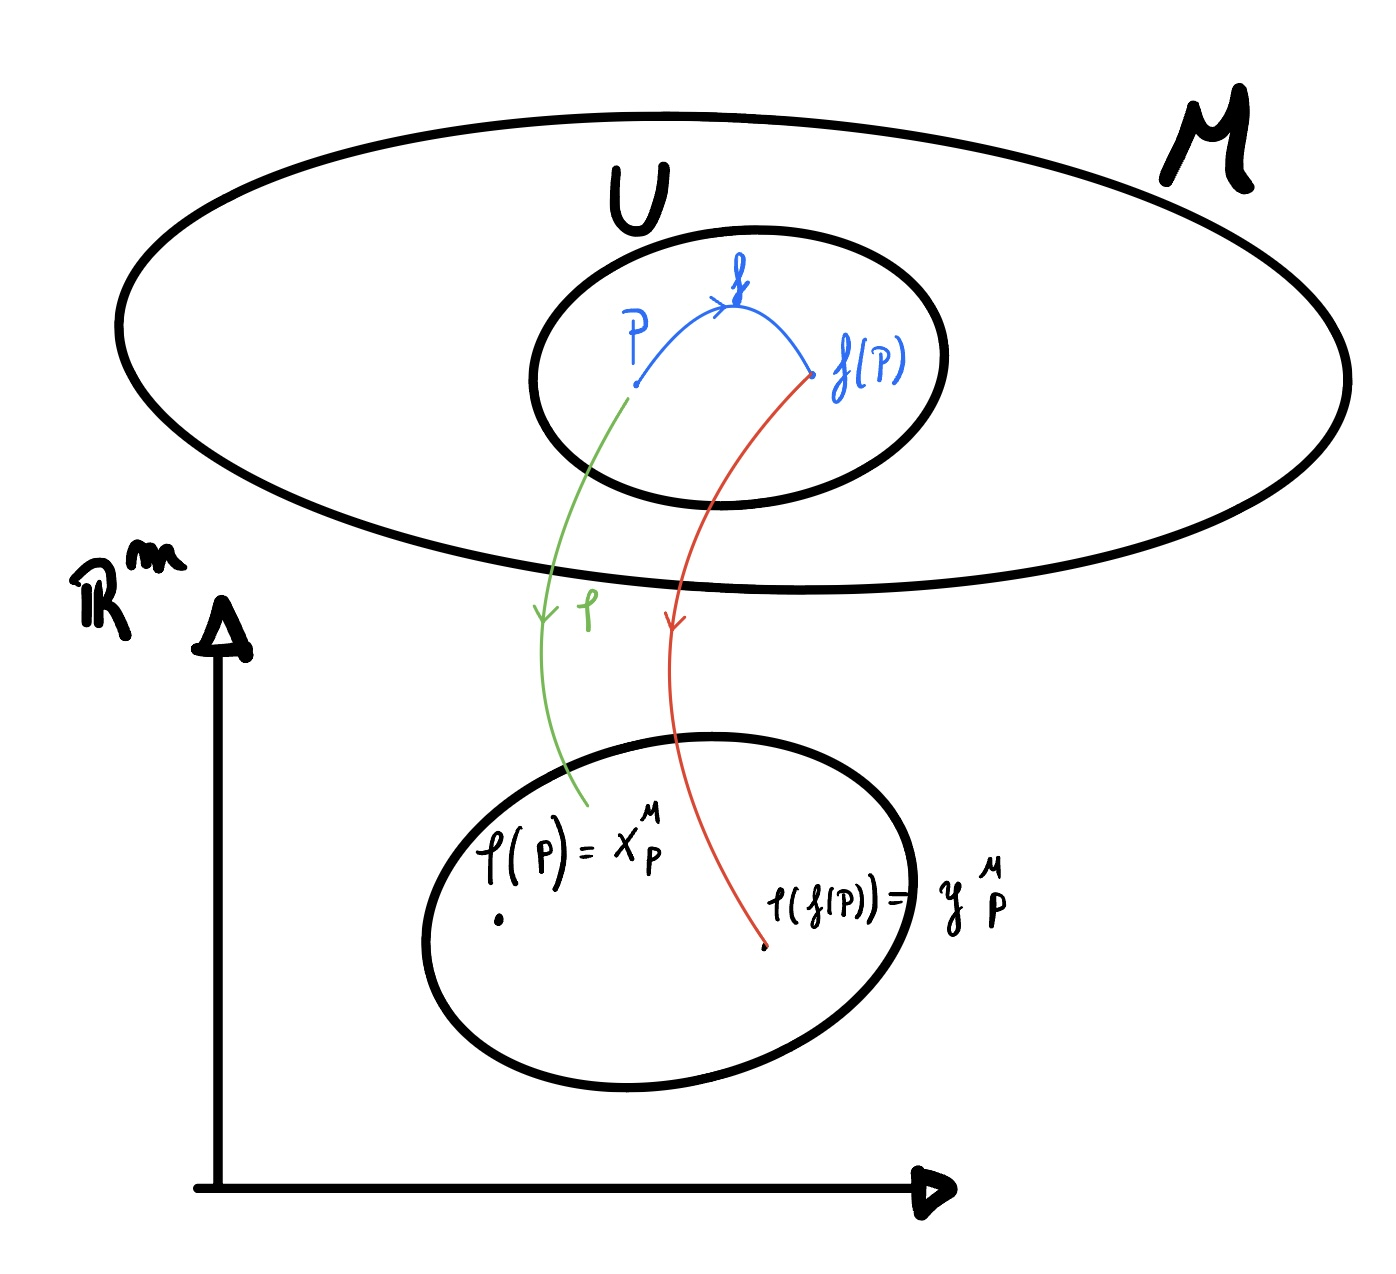
\includegraphics[scale=0.15]{Chapitres/3.Element de géométrie différentielle/Images/transformation actives.jpg}
%\captionof{figure}{}
%\label{Parabolique 2}
\end{center}
\item Soient deux cartes locales de $P$, notées $(U,\varphi)$ et $(V,\psi)$ et notons $\varphi(P) = x^\mu(P)$ et $\psi(P) = y^\mu(P)$. Remarquons que ces deux coordonnées ne coïncident pas nécessairement. Ils sont, liés par la fonction de transition $f = \varphi \circ \psi^{-1}, \, y^\mu \mapsto x^\mu$, qui est un difféomorphisme. Cette représentation est nommée \emph{transformation passive des coordonnées}, car le point $P$ reste le même : la différence vient des deux cartes distinctes utilisées.
\end{enumerate}

\subsection{Un atlas pour $S^2$}
Nous nous chargerons d'illustrer un cas où une carte globale n'existe pas\footnote{Il est un exercice intéressant de montrer qu'une paramétrisation globale n'existe pas. Une intuition peut être donné par le théorème de la boule chevelue.}. Le cas le plus simple est la 2-sphère définie par 
\begin{equation}
    S^2 \equiv \{ (x,y,z) \in \R^3 \mid x^2+y^2+z^2 = 1\}
\end{equation}
Nous allons construire un atlas de $S^2$. Pour ce, nous allons utiliser la \emph{projection stéréographique} : Soit le pôle nord $N = (0,0,1)$. Remarquons que pour tout point $P\in S^2\backslash \{N\}$, il existe une unique droite passant par $P$ et $N$. La projection stéréographique $\varphi_N:S^2\backslash\{N\} \to \R^2$ de $P$ par rapport à $N$ est alors définie comme l'intersection de cette droite avec le plan $z=0$. Selon cette définition, le pôle sud $S = (0,0,-1)$ est envoyé sur $(0,0)$, et lorsque $P \to N$, $\lVert \varphi(P) \lVert \to \infty$.

\begin{figure}[H]
    \centering
    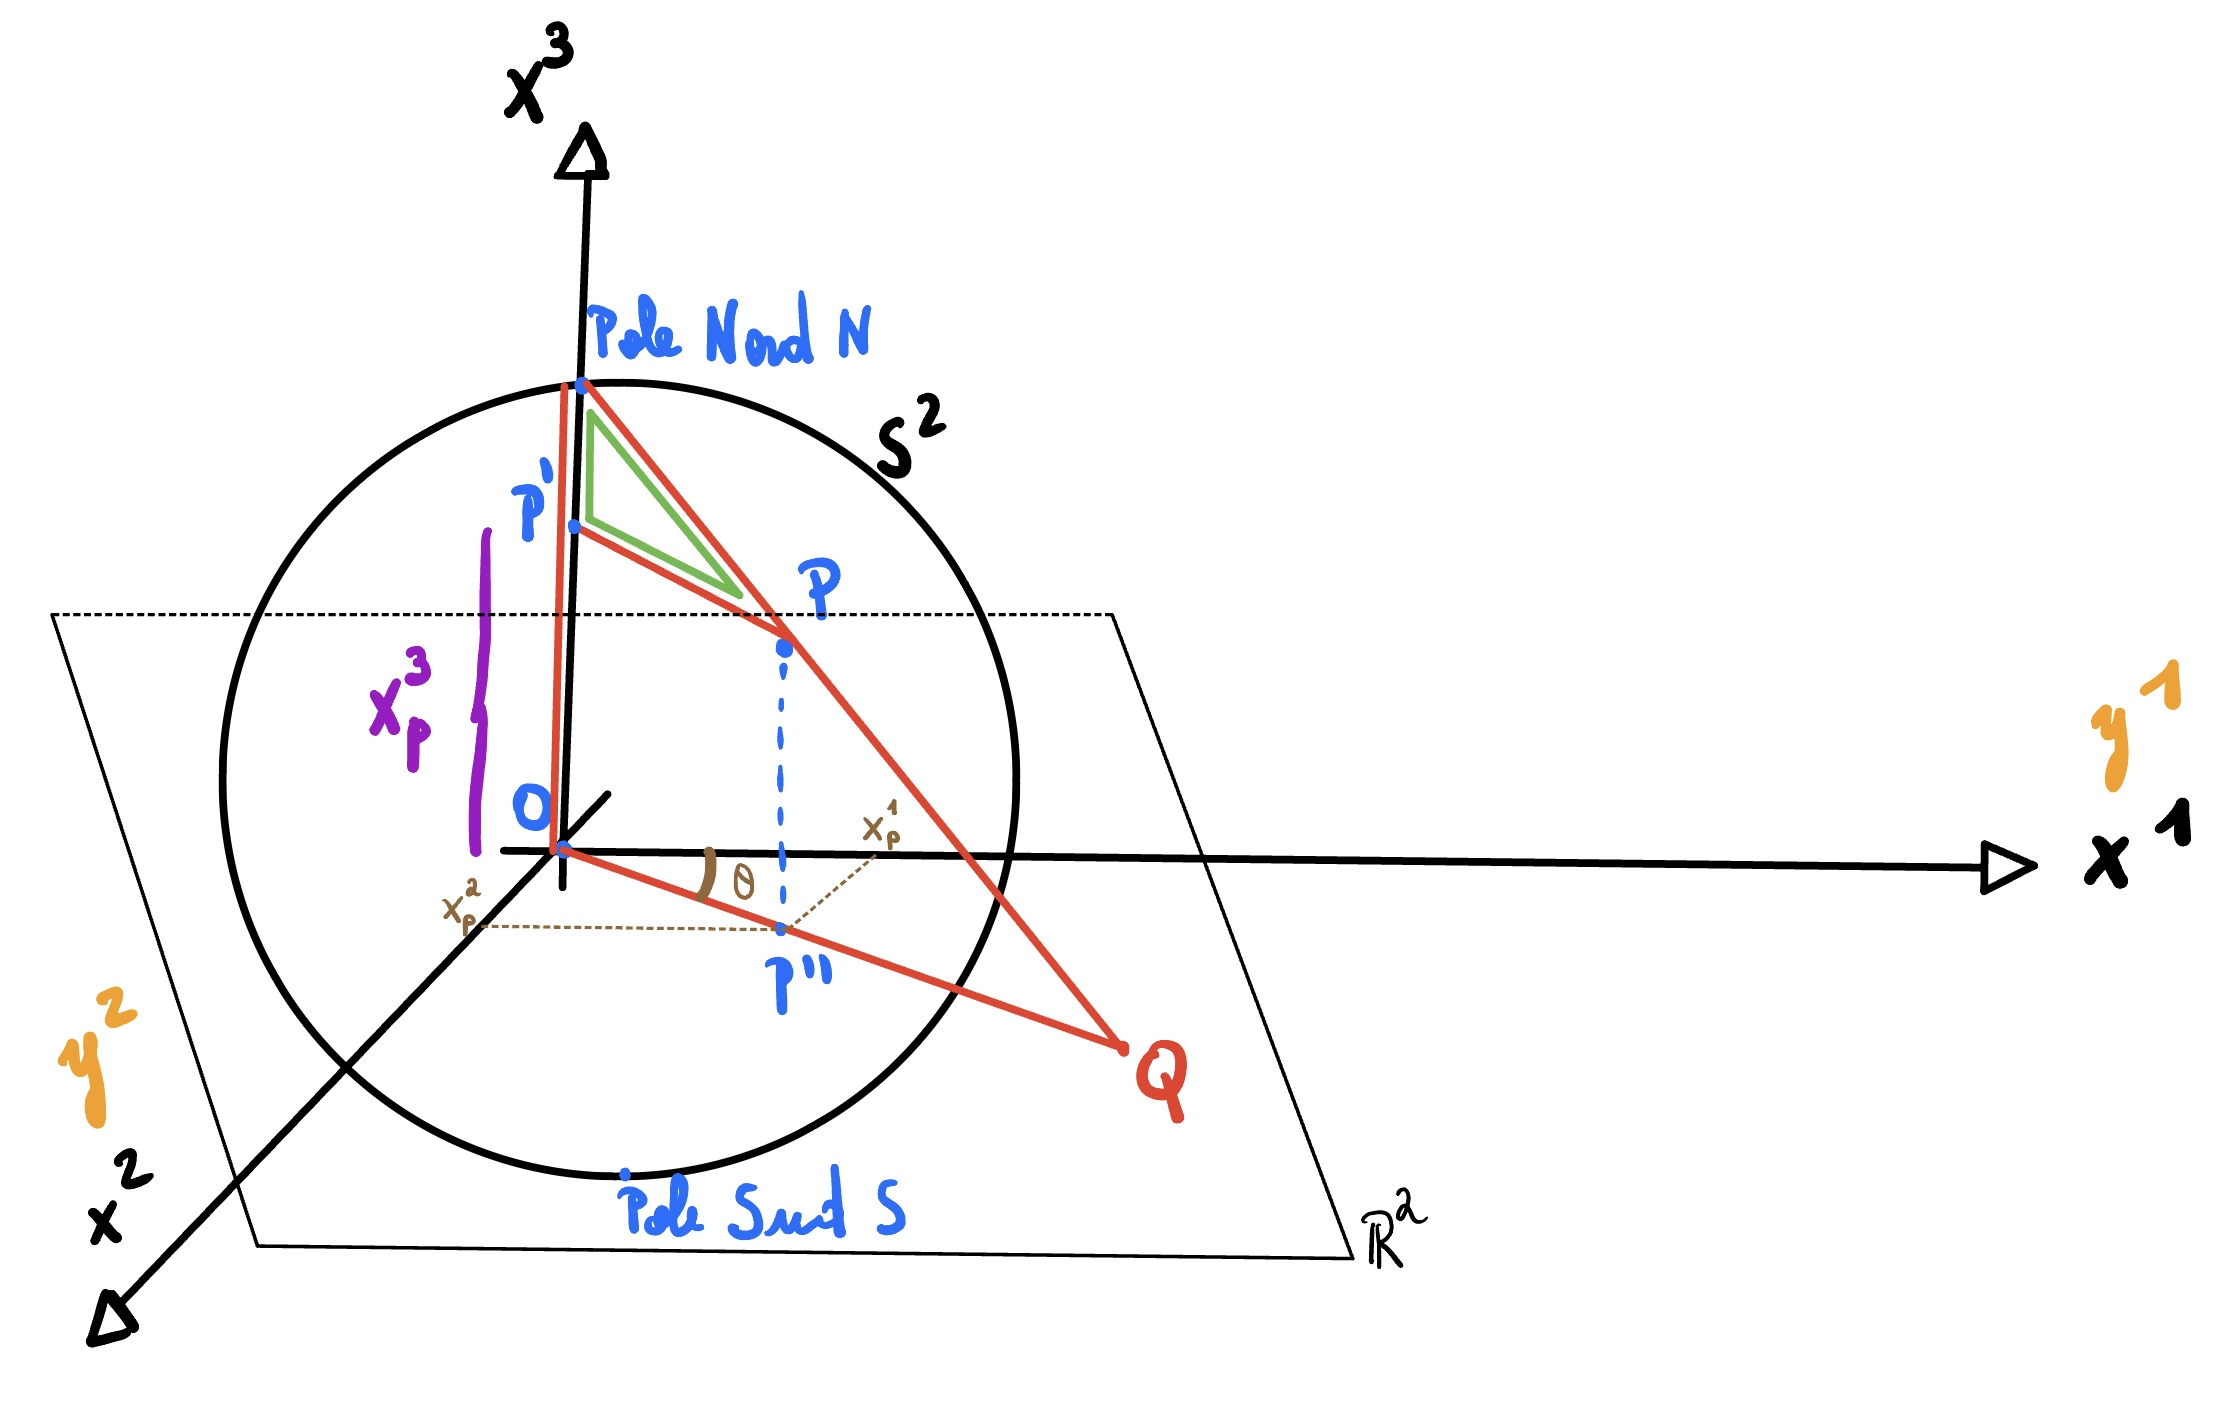
\includegraphics[width=0.7\linewidth]{Chapitres/3.Element de géométrie différentielle/Images/sphère S^2.jpg}
    \caption{Visualisation de la projection stéréographique par rapport à $N$.}
    \label{fig:stereographique 1}
\end{figure}

Dérivons la forme explicite pour $\varphi_N$. Notons $O = (0,0,0)$ et considérons un point $P\in S^2$ ainsi que sa projection stéréographique $Q \in R^2 \times \{0\}$. Notons de plus $P_z$ la projection de $P$ sur l'axe $\vect{u}_z$ et $P_{xy}$ la projection de $P$ sur le plan $Oxy$. Remarquons que les triangles $PP_zN$ et $QON$ sont semblables et donc
\begin{align}
    \frac{OQ}{ON} = \frac{P_zP}{NP_z} \implies OQ = \frac{OP_{xy}}{1-x^3_P}
\end{align}
car $ON = 1$, $P_zP = OP_{xy}$ et $NP_z = 1 - x^3_P$. Finalement, on trouve donc que 
\begin{equation}
    Q^i = \varphi_N(P)^i = \frac{x^i_P}{1-x^3_P}
\end{equation}
où $i=1,2$. La 
\begin{equation}
\label{eq:stereoN}
    \varphi_N : S^2\backslash\{N\} \to \R^2 : (x^1,x^2,x^3) \mapsto \frac{1}{1-x^3} (x^1,x^2)
\end{equation}
Similairement, la projection stéréographique par rapport au pôle sud est
\begin{equation}
    \label{eq:stereoS}
    \varphi_S:S^2\backslash \{S\} \to \R^2 : (y^1,y^2,y^3) \mapsto \frac{1}{1+y^3} (y^1,y^2)
\end{equation}
Montrons à présent que $\{ (S^2\backslash\{N\}, \varphi_N), (S^2\backslash\{S\}, \varphi_S)\}$ est un atlas lisse de $S^2$. Pour ce, nous devons montrer que les fonctions de transitions sont lisses. Posons $\varphi_N^i = z^i$. On a alors
\begin{equation}
\label{eq:1 altasS2}
    z^i = \frac{x^i}{1-x^3}
\end{equation}
Et en utilisant la définition de $S^2$ :
\begin{equation}
    (z^1)^2 + (z^2)^2 = \frac{1 - (x^3)^2}{(1-x^3)^2} = \frac{1 + x^3}{1-x^3}
\end{equation}
Ceci nous permet d'isoler et de réinjecter $x^3$ dans (\ref{eq:1 altasS2}). On trouve alors
\begin{equation}
    \psi_N = \varphi_N^{-1}: \R^2 \to S^2\backslash \{N\}:(u,v) \mapsto \frac{1}{1+u^2 +v^2} \lt 2 u,2v, -1 + u^2+v^2 \rt
\end{equation}
La fonction de transition est alors
\begin{align}
    \varphi_S \circ \psi_N : \psi^{-1}_N \circ \varphi^{-1}_S(\R^2) = \R^2_0 \to \R^2 : (u,v) \mapsto \frac{(u,v)}{u^2+v^2}
\end{align}
Qui est lisse sur $\R^2_0$. Remarquons que $\psi_N(0,0) = (0,0,-1)=S$, donc notre domaine de définition est bien correct (comme $\varphi_S$ n'est pas définie en $S$, nous devons exclure $(0,0)$ du domaine).
\begin{exerc}
    Dérivez l'expression (\ref{eq:stereoS}) pour $\varphi_S : S^2\backslash \{ S\} \to \R^2$. Calculez $\psi_S$ et montrez que $\varphi_N \circ \varphi_S^{-1}$ est bien lisse sur son domaine. 
\end{exerc}
Nous avons trouvé un atlas lisse de $S^2$.
\section{Vecteurs dans une variété}
Nous devons retravailler la notion de vecteur introduite à la section 1.1, afin qu'elle soit intrinsèque à $\mathcal{M}$. Le problème principal est qu'une variété arbitraire n'est pas un espace vectoriel, seulement le plan tangent en est un. Fixons un point $m\in \mathcal{M}$ ($\dim \mathcal{M} = n$) et une courbe $\gamma$ dans $\mathcal{M}$ telle que $\gamma(0)=m$.
\begin{theoremframe}
    \begin{defi}
        Un \emph{vecteur tangent} $X_m$ à $\mathcal{M}$ en $m$ est un opérateur différentiel linéaire agissant sur les fonctions lisses dans un voisinage de $m$ tel que
        \begin{equation}
        \label{eq: vectvar}
            X_m f =\left. \frac{\td}{\td \lambda}\right|_{\lambda=0}  f \circ \gamma(\lambda)
        \end{equation}
    \end{defi}
\end{theoremframe}
Un vecteur tangent peut donc être vu comme une dérivée directionnelle s'appliquant sur les fonctions le long d'une courbe en $\lambda=0$. Nous abuserons parfois de cette notation en écrivant $X = \frac{\td}{\td \lambda}$. Notons que (\ref{eq: vectvar}) s'écrit en composantes :
\begin{equation}
    X_i f = \left. \frac{\td}{\td \lambda}\right|_{\lambda=0}  f \circ \gamma_i(\lambda).
\end{equation}
Soit une carte locale $(U,\varphi)$ de $\mathcal{M}$ au point $m$. Notons $F = f \circ \varphi^{-1} : \R^m\to \R$ et $x^\mu(\gamma) = \varphi \circ \gamma: \R \to \R^m$ les représentations en coordonnées de $f$ et $\gamma$ dans cette carte locale. On trouve alors
\begin{align}
    X_m f = \left. \frac{\td}{\td \lambda}\right|_{\lambda=0}  f \circ \gamma(\lambda) &= \left. \frac{\td}{\td \lambda}\right|_{\lambda=0}  f \circ \varphi^{-1} \circ \varphi \circ \gamma(\lambda)\\
    & = \left. \frac{\td}{\td \lambda}\right|_{\lambda=0}  F \circ x^\mu(\gamma((\lambda))
\end{align}
S'agissant à présent de fonctions dans des espaces euclidiens, nous pouvons appliquer la règle de la chaine.
\begin{align}
    X_mf = \left. \frac{\pd F}{\pd x^\mu} \right|_{x^\mu=x^\mu(m)} \left. \frac{\pd x^\mu}{\pd \lambda} \right|_{\lambda = 0} (\gamma(\lambda))
\end{align}
En omettant la différence entre la fonction $f$ et sa représentation locale $F$, nous écrirons
\begin{align}
    X_m f = \left. \frac{\td}{\td \lambda} \right|_{\lambda=0} f = \left. \frac{\td x^\mu}{\td \lambda} \right|_{\lambda = 0} \frac{\pd}{\pd x^\mu}f
\end{align}
Comme $f$ est arbitraire, nous trouvons
\begin{equation}
    X_m = \left. \frac{\td x^\mu}{\td \lambda} \right|_{\lambda = 0} \frac{\pd}{\pd x^\mu}
\end{equation}
où les premiers termes sont les composantes du vecteur $X_m$ et les deuxièmes termes $\{\pd_\mu \}$ forment une base de l'espace $T_m\mathcal{M}$. Remarquons que donc, la dimension de $T_m\mathcal{M}$ est $n$.
\begin{center}
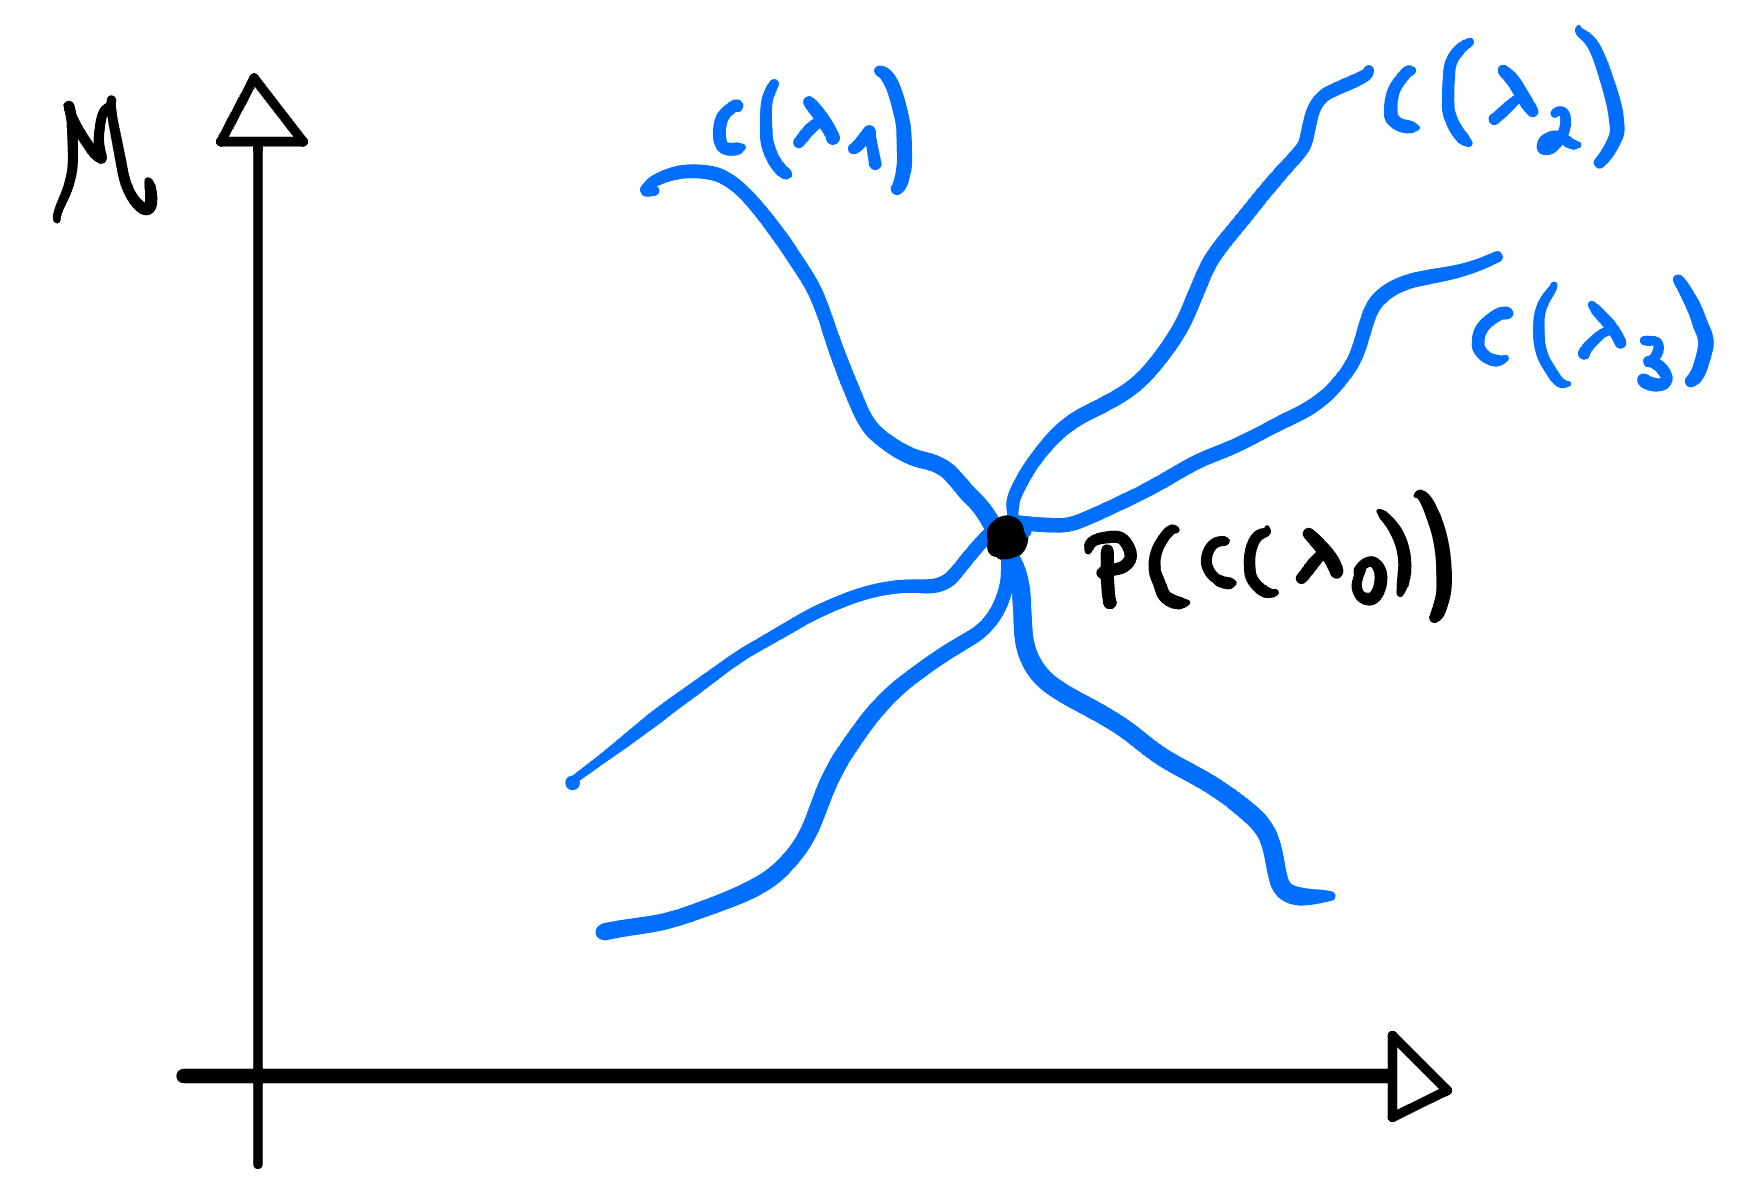
\includegraphics[scale=0.1]{Chapitres/3.Element de géométrie différentielle/Images/vecteurs2.0.jpg}
%\captionof{figure}{}
%\label{Parabolique 2}
\end{center}


\begin{center}
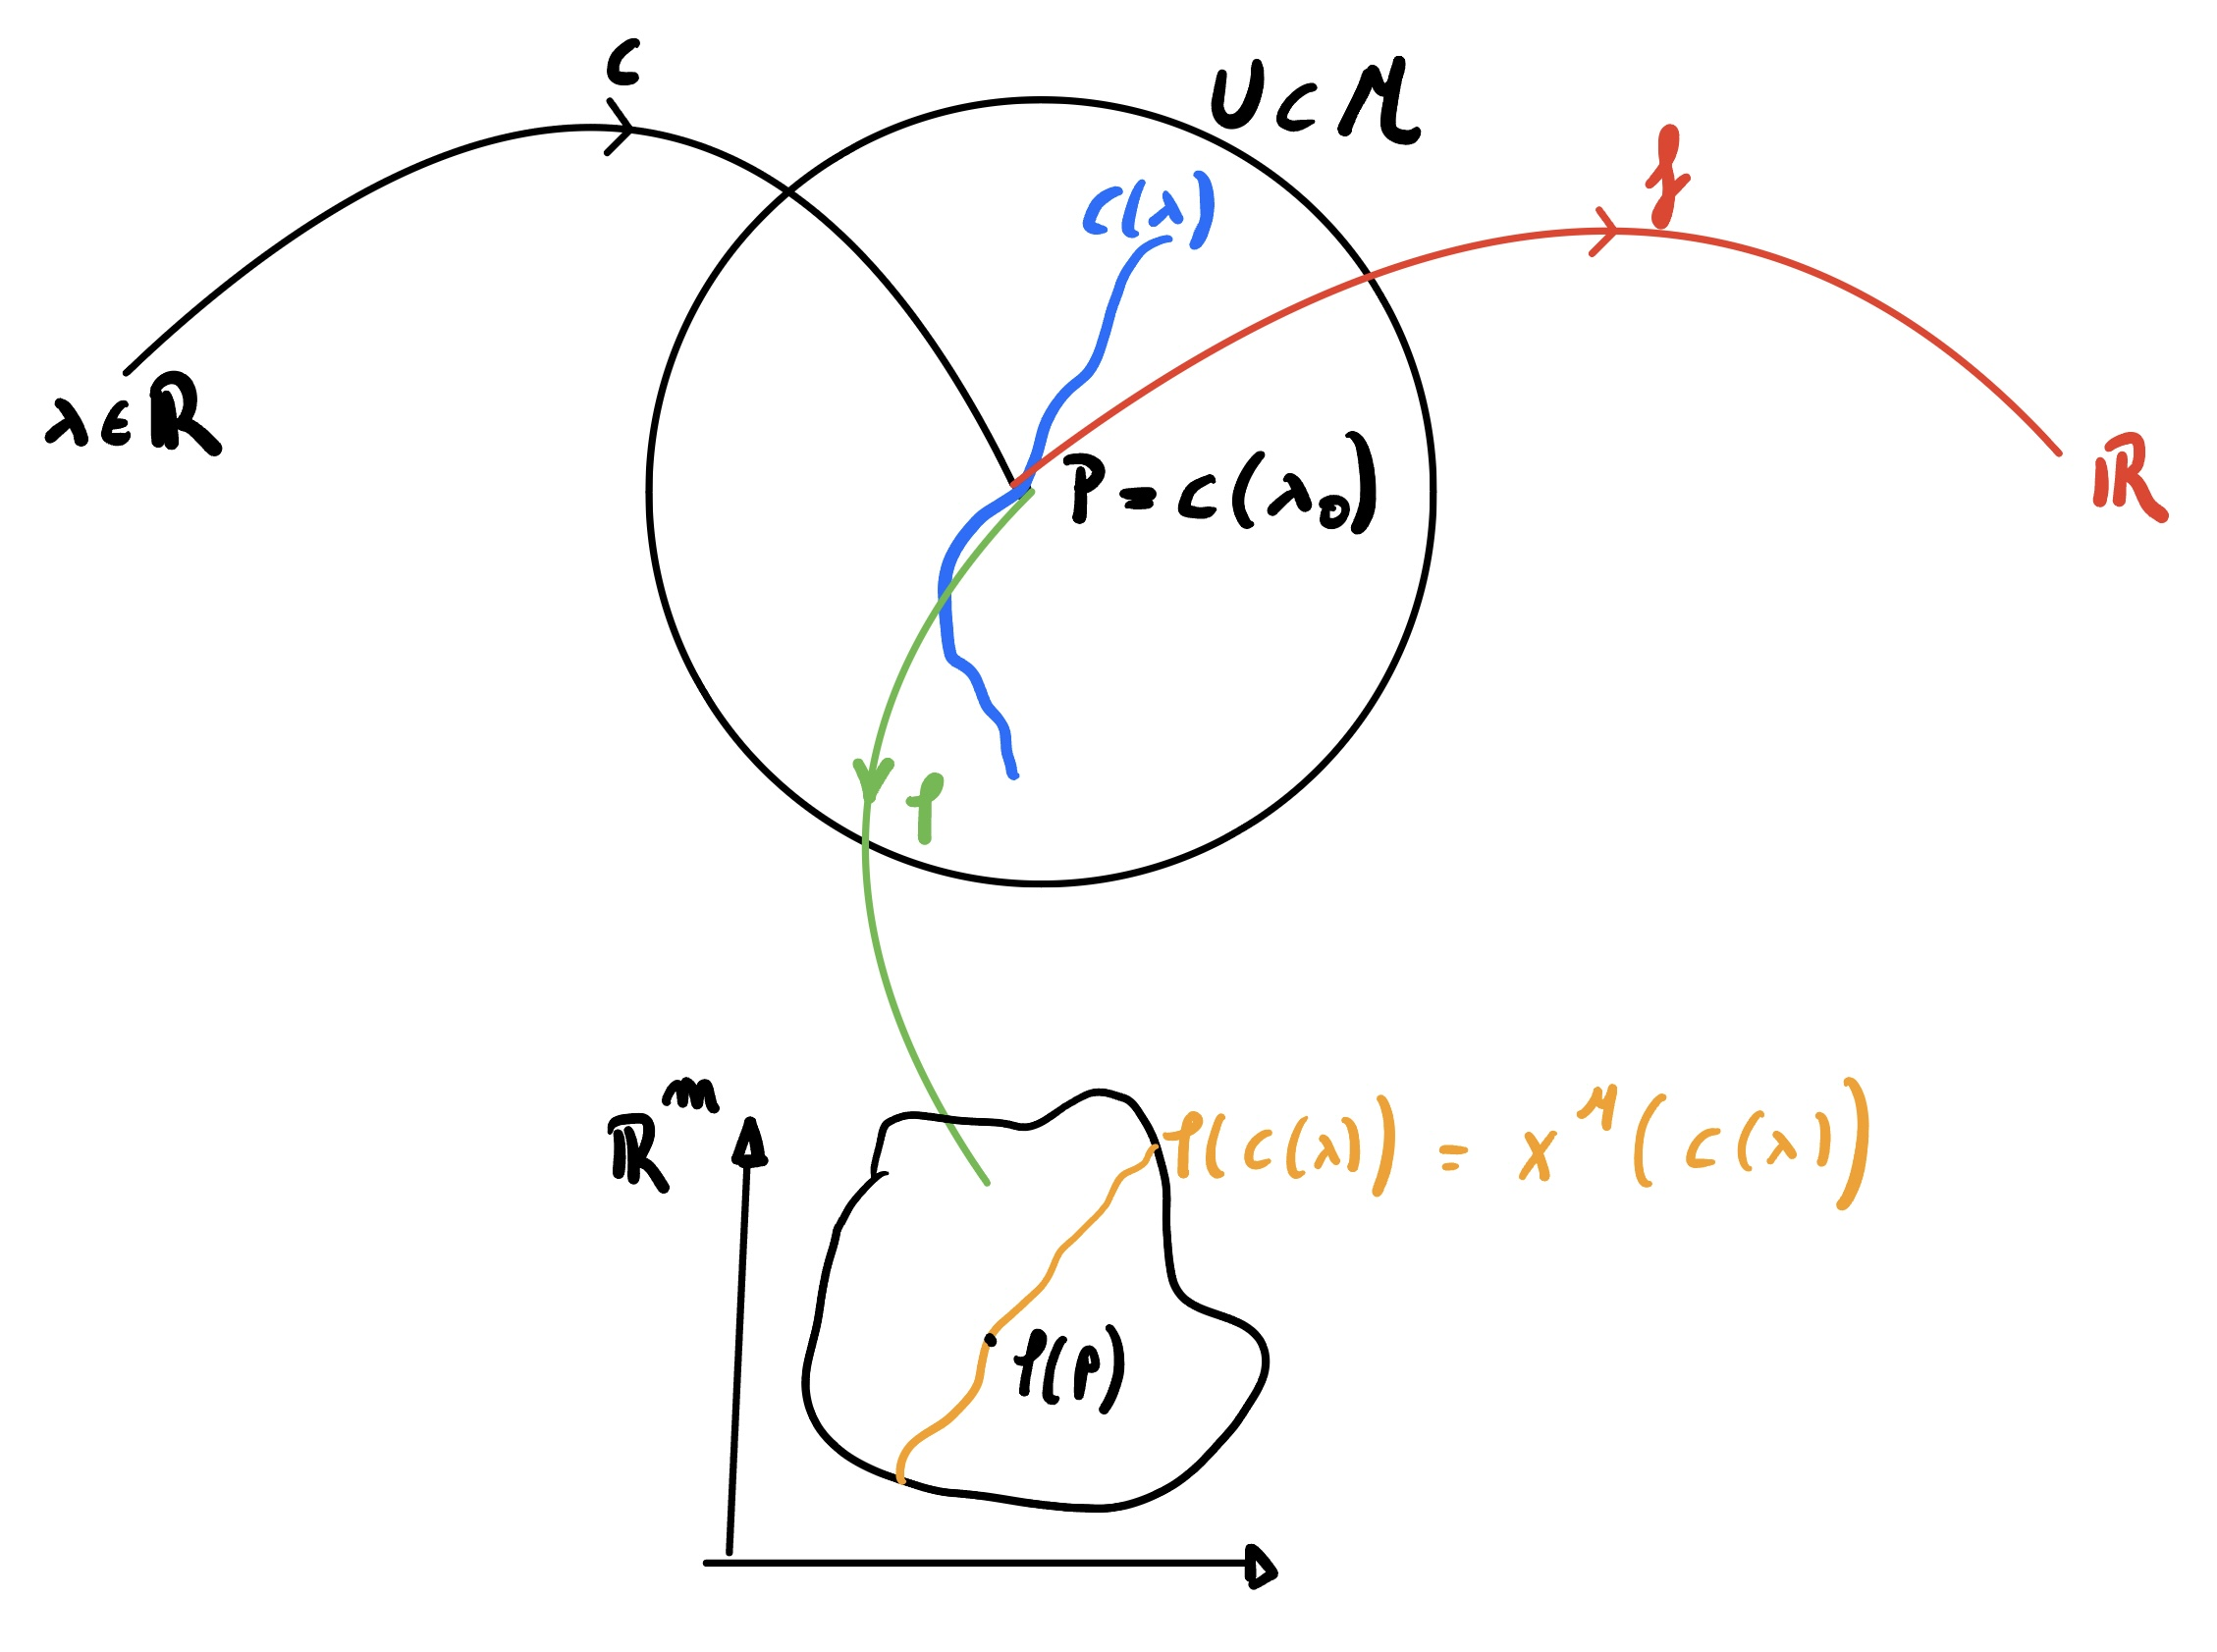
\includegraphics[scale=0.1]{Chapitres/3.Element de géométrie différentielle/Images/dimenson.jpg}
%\captionof{figure}{}
%\label{Parabolique 2}
\end{center}


De manière plus concise, on notera

\begin{equation*}
    X = \frac{\td}{\td \lambda }= \frac{\td x^{\mu}}{\td \lambda } \frac{\partial }{\partial x^{\mu}} = X^{\mu} \partial_{\mu}
\end{equation*}

où nous sous-entendons $x^{\mu} = x^{\mu}( \gamma(\lambda))$. Les vecteurs $X = \pd_\mu$ représentent un déplacement tangent à la direction $x^\mu$. Contrairement à la variété $\mathcal{M}$, qui n'est pas un espace vectoriel dans le cas général, l'espace tangent en est un. 
\begin{center}
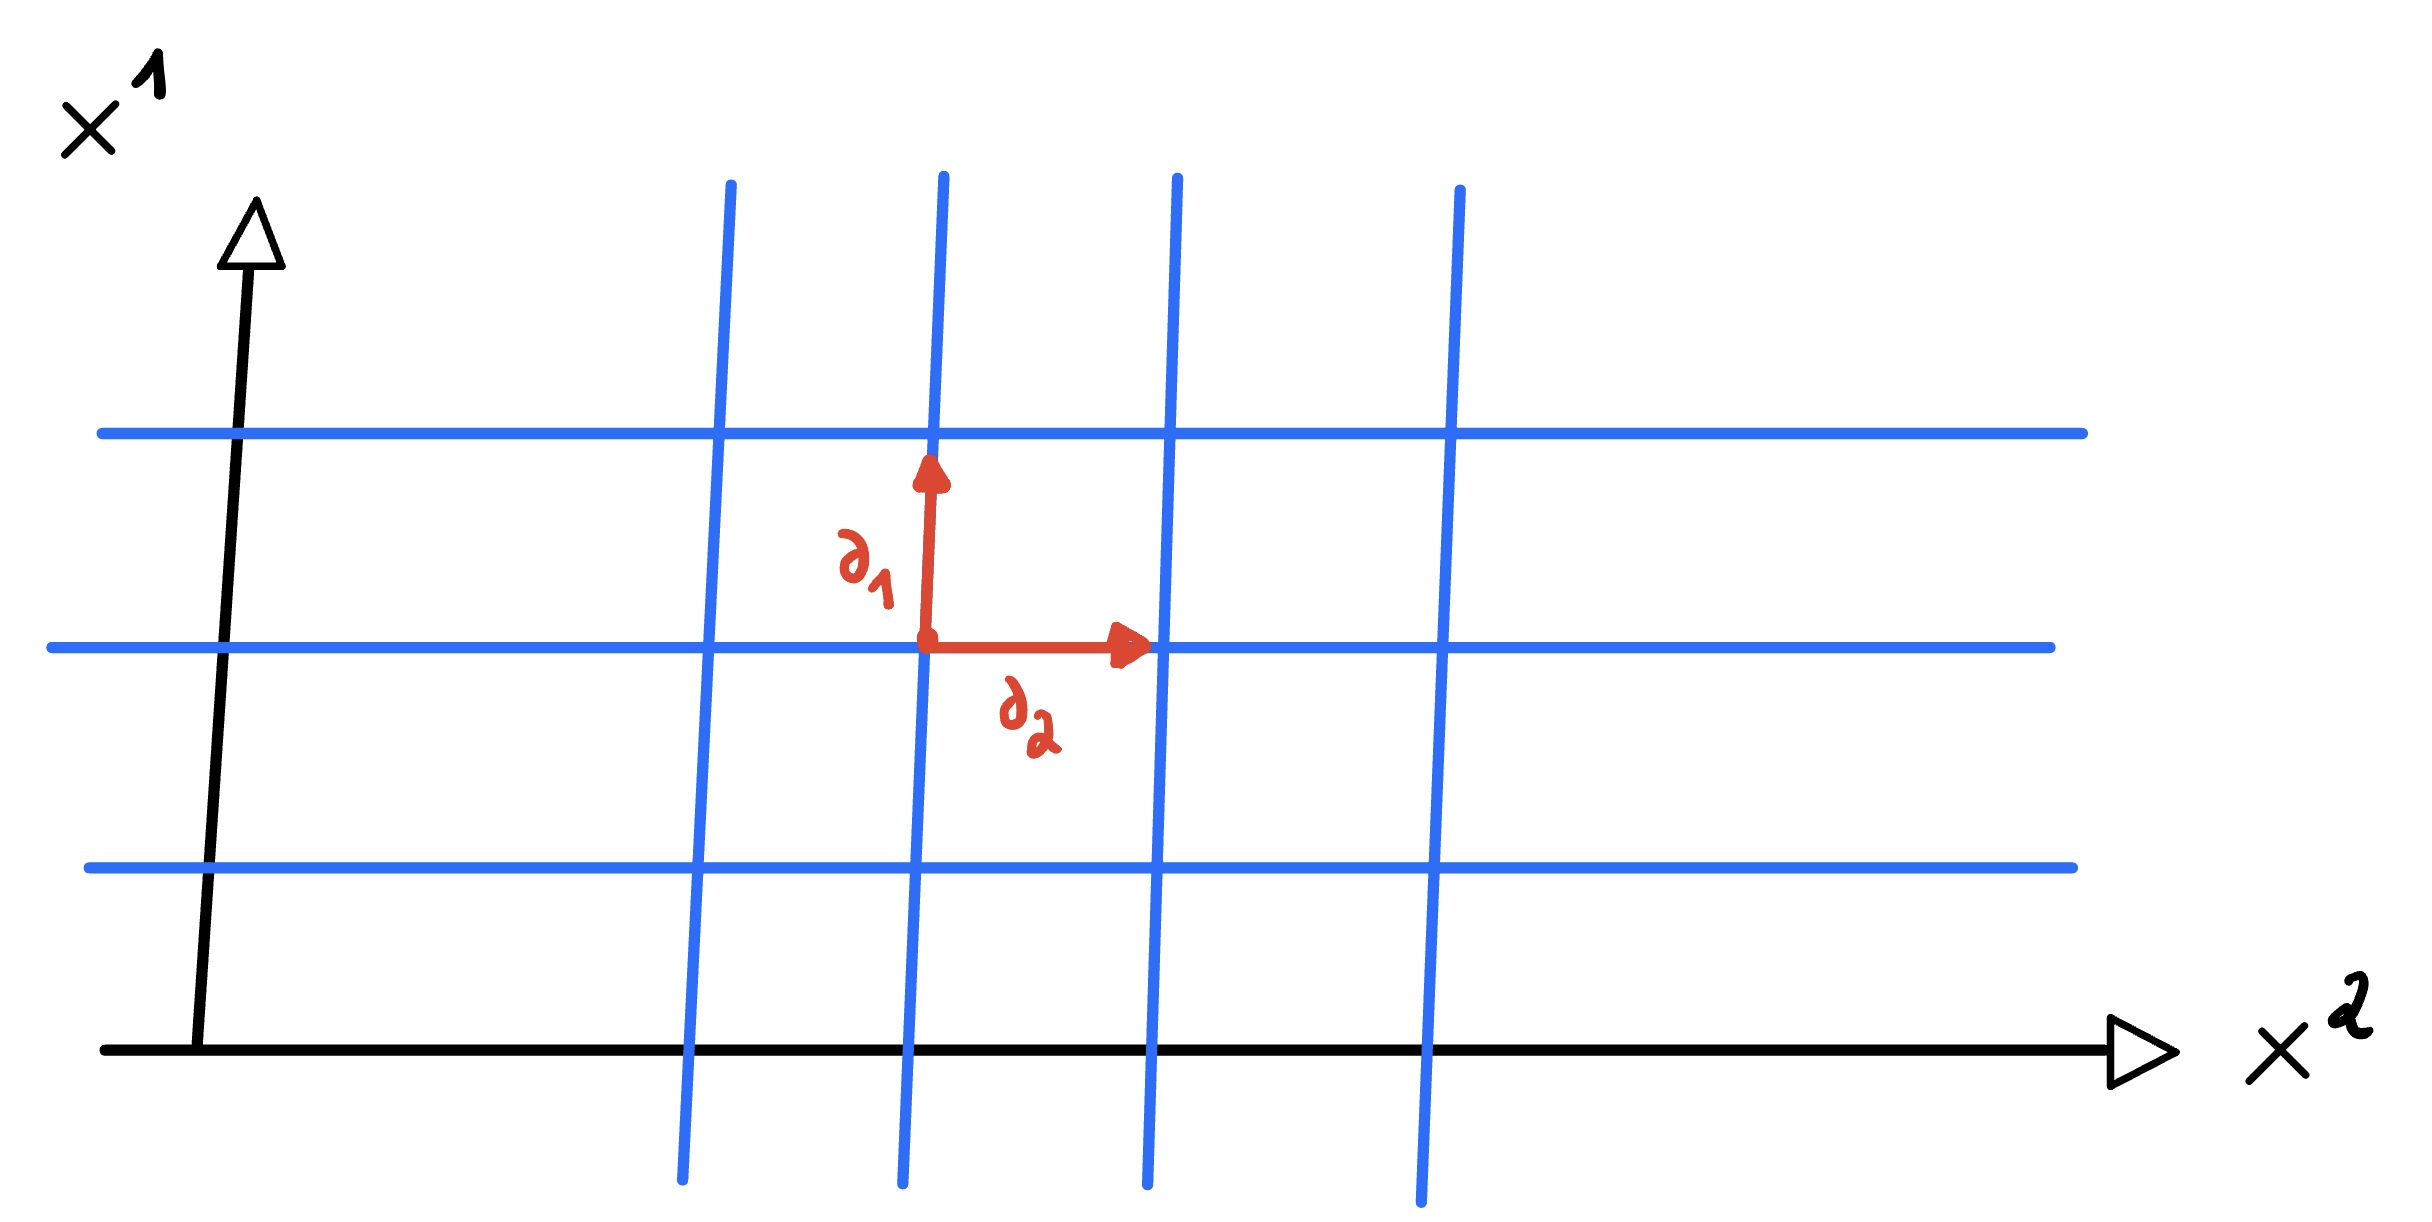
\includegraphics[scale=0.1]{Chapitres/3.Element de géométrie différentielle/Images/vecteur-fleche.jpg}
%\captionof{figure}{}
%\label{Parabolique 2}
\end{center}
\subsubsection{Loi de transformation des vecteurs}
Les vecteurs sont indépendants de la base et du choix de la carte locale. Sous changement général de coordonnées (difféomorphisme), les composantes $X_\mu$ d'un vecteur se transforment selon
    \begin{align}
        \boxed{X^\mu \to X^{\mu'} = \frac{\td x^{\mu'}}{\td \lambda} = \frac{\pd x^{\mu'}}{\pd x^\alpha} \frac{\td x^\alpha}{\td \lambda} = \frac{\pd x^{\mu'}}{\pd x^\alpha} X^\alpha}
    \end{align}
Similairement, les vecteurs de base se transforment selon
\begin{equation}
    \pd_\alpha \to \pd_{\alpha'} = \frac{\pd x^\mu}{\pd x^{\alpha'}} \pd_\mu
\end{equation}
de sorte que $X$ soit invariant sous difféomorphisme. Remarquons qu'il s'agit ici simplememnt de la règle de la chaîne. Notons les identités suivantes de la jacobienne $\frac{\pd x^{\mu'}}{\pd x^\alpha}$.
\begin{align}
    \label{eq: id chgmt de coordonnées}
    \boxed{
        \begin{array}{c}
            \displaystyle
            \dfrac{\pd x^{\mu'}}{\pd x^\alpha}\dfrac{\pd x^{\beta}}{\pd x^{\mu'}} = \displaystyle \delta^\beta_\alpha  \\
            \\
            \dfrac{\pd x^{\alpha}}{\pd x^{\nu'}}\dfrac{\pd x^{\mu'}}{\pd x^\alpha} =\displaystyle\delta\indices*{^{\mu'}_{\nu'}}
        \end{array} 
    }
\end{align}
\begin{exerc}
    Démontrez ces égalités.
\end{exerc}
Pour récapituler, nous avons trouvé qu'un vecteur dans $T_m\mathcal{M}$ peut être vu comme une application
\begin{equation}
    X_m:C^\infty(U) \to \R:f \mapsto X_m f = \left. X^\mu_m \pd_\mu f \right|_{x^\mu(m)}
\end{equation}
où $U$ est un voisinage de $m$. Nous définirons par ailleurs un champ de vecteurs comme la donnée d'un vecteur en tout point $m \in \mathcal{M}$.
\begin{equation}
    \chi: T\mathcal{M} \to \R
\end{equation}
Où $T\mathcal{M}$ est le fibré tangent. Le champ de vecteurs est dit lisse s'il dépend lissement du point $m$ (dans le sens des représentations locales de coordonnées). L'ensemble des champs de vecteurs lisses sur $\mathcal{M}$ est noté $ \Zhe (\mathcal{M})$.

\subsection{Covecteurs}

Soit $X_m \in T_m \mathcal{M}$. Un covecteur $w\in T_m^*\mathcal{M}$ est une forme linéaire sur $T_m\mathcal{M}$ 
\begin{equation}
w  : T_m \mathcal{M} \rightarrow \R : X \mapsto w(X)
\end{equation}
où pour rappel l'espace $T^*_m \mathcal{M}$ est le dual de $T_m\mathcal{M}$, également appelé l'espace cotangent. 

\begin{exmp}
    Soit $f\in C^\infty(\mathcal{M})$. La différentielle $\td f$ de $f$ au point $m\in \mathcal{M}$ est un covecteur. Son action est définie par
    \begin{equation}
        \left. \td f \right|_m : T_m \mathcal{M} \to \R : \td f (X) = X(f) = \left. X^\mu_m \pd_\mu f \right|_m.
    \end{equation}
On se souviendra qu'une base de l'espace cotangent est donnée par $\{ \td x^\nu\}$. Nous avions également trouvé que la relation entre la base de l'espace tangent et de l'espace cotangent est
\begin{equation}
    \td  x^\mu (\pd_\nu) = \delta\indices*{^\mu_\nu}
\end{equation}
Suivant notre définition de covecteur, nous pouvons à présent justifier cette relation. En effet, soit $X = \pd_\nu$. Alors
\begin{equation}
    \td x^\mu \lt \frac{\pd}{\pd x^\nu}\rt \equiv \frac{\pd}{\pd x^\nu}(x^\mu) = \delta\indices*{^\mu_\nu}
\end{equation}
Dans une carte locale, nous décomposer $\td f$ sur la base selon
\begin{equation}
    \td f = \frac{\pd f}{\pd x^\mu} \td x^\mu
\end{equation}
\end{exmp}
Montrons à présent que selon notre définition, $w(X)$ est bien scalaire. Dans une carte locale, on a
\begin{equation}
    w(X) = w_\mu \td x^\mu (X^\nu \pd_\nu ) = w_\mu X^\nu \td x^\mu (\pd_\nu) = w_\mu X^\nu \delta\indices*{^\mu_\nu} = w_\mu X^\mu
\end{equation}
Où nous avons utilisé la linéarité de $\td x^\mu$. On conclut que $w(X)$ est bien un scalaire. Sous changements de coordonnées général (difféomorphisme), on trouve donc via l'invariance de $w(X)$ et la loi de transformation de $X$ que
\begin{equation}
    w_\mu X^\mu = w_{\mu'} X^{\mu'} = w_{\mu'} \frac{\pd x^{\mu'}}{\pd x^\mu} X^\mu
\end{equation}
Où on peut donc identifier
\begin{equation}
    w_\alpha = w_{\alpha'} \frac{\pd x^{\alpha'}}{\pd x^\alpha}
\end{equation}
En inversant cette relation via (\ref{eq: id chgmt de coordonnées}), on obtient finalement la loi de transformation sous changement de coordonnées général pour un covecteur

 \begin{equation}
     \boxed{w_\mu \to w_{\mu '} = \frac{\partial x^{\alpha }}{\partial x^{\mu '}} w_{\alpha}}
 \end{equation}

Les vecteurs de bases se transforment comme

$$dx^{\mu'} = \frac{\partial x^{\mu'}}{\partial x^{\alpha}} dx^{\alpha}$$
\subsection{Les tenseurs généraux}
Comme nous nous intéresserons exclusivement à des espaces à dimension finie, $(T^*_m \mathcal{M})^* \simeq T_m \mathcal{M}$ : les vecteurs peuvent êtres vues comme formes linéaires sur l'espace cotangent.
\begin{equation}
    V: T^*_m \mathcal{M} \to \R : w \mapsto V(w) \equiv w(V )
\end{equation}
Soit un point $m\in \mathcal{M}$
\begin{theoremframe}
    \begin{rap}
        \label{rap:tenseur}
        Un \emph{tenseur} de type $(p,q)$ est une forme multilinéaire 
        \begin{equation}
            \underbrace{T^*_{m}\mathcal{M} \times \cdots \times T^*_{m}\mathcal{M}}_\text{$p$-fois} \times \underbrace{T_{m}\mathcal{M} \times \cdots \times T_{m}\mathcal{M}}_\text{$q$-fois}  \to \mathbb{R}
        \end{equation}
    \end{rap}
\end{theoremframe}
\begin{exmp} Donnons quelques exemples\\
    \begin{enumerate}
        \item Un \emph{vecteur} est un objet 
        \begin{equation}
            X:T_m^*\mathcal{M} \to \R
        \end{equation}
        et est donc un tenseur $(1,0)$. Dans une carte locale, celui-ci s'écrit $X^\mu \pd_\mu$. Remarquons qu'on a bien $X(\omega) \in \R$.
        \item Un \emph{covecteur} est un objet 
        \begin{equation}
            w:T_m\mathcal{M} \to \R
        \end{equation}
        et est donc un tenseur $(0,1)$. Dans une carte locale, celui-ci s'écrit $w_\mu \td x^\mu$.
        \item De manière générale, les composantes d'un tenseur quelconque $(p,q)$ possèdent $p$ indices contravariants et $q$ indices covariants. Dans une carte locale, le tenseur s'écrit
        \begin{equation}
            T = T\indices{^{\alpha_1} ^{\cdots}^{\alpha_p}_{\nu_1}_{\cdots} _{\nu_q}} \partial_{\alpha_{1}}
            \otimes ... \otimes \partial_{\alpha_{p}} \otimes dx^{\nu_{1}}\otimes...\otimes dx^{\nu_{q}} 
        \end{equation}
        Ses composantes se transforment sous changement de coordonnées général selon
        \begin{equation}
            T\indices{^{\alpha_1} ^{\cdots}^{\alpha_p}_{\nu_1}_{\cdots} _{\nu_q}} \to T\indices{^{\alpha'_1} ^{\cdots}^{\alpha'_p}_{\nu'_1}_{\cdots} _{\nu'_q}} = \frac{\partial x^{\alpha'_1}}{\partial x^{\alpha_1}} \cdots\frac{\partial x^{\alpha'_p}}{\partial x^{\alpha_p}}\frac{\partial x^{\nu_1}}{\partial x^{\nu'_1}}\cdots\frac{\partial x^{\nu_q}}{\partial x^{\nu'_q}} T\indices{^{\alpha_1} ^{\cdots}^{\alpha_p}_{\nu_1}_{\cdots} _{\nu_q}}
        \end{equation}
    \end{enumerate}
\end{exmp}
\section{Les p-formes différentielles}
Nous souhaitons pouvoir définir une structure différentielle sur notre variété, c'est-à-dire construire une manière de différentier un tenseur quelconque sur notre variété, qui nous permettrait d'étudier des systèmes dynamiques dans notre variété (i.e. des équations différentielles). Or, un problème apparaît lorsqu'on s'intéresse à la quantité $\pd_\mu w_\nu$. Sous changement général de coordonnées, cette quantité varie selon
\begin{align}
\nonumber
    \label{eq: not a tensor}
    \pd_\mu w_\nu \to \pd_{\mu'} w_{\nu'} &= \frac{\pd x^\mu}{\pd x^{\mu'}} \pd_\mu \lt \frac{\pd x^\nu}{\pd x^{\nu'}} w_\nu \rt\\
    & = \frac{\pd x^\mu}{\pd x^{\mu'}} \frac{\pd x^\nu}{\pd x^{\nu'}} \pd_\mu w_\nu + \frac{\pd x^\mu}{\pd x^{\mu'}} w_\nu \frac{\pd}{\pd x^\mu}  \frac{\pd x^\nu}{\pd x^{\nu'}}\\
    \nonumber
    &= \frac{\pd x^\mu}{\pd x^{\mu'}} \frac{\pd x^\nu}{\pd x^{\nu'}} \pd_\mu w_\nu + w_\nu  \frac{\pd^2 x^\nu}{\pd x^{\mu'}\pd x^{\nu'}}
\end{align}
Où nous avons utilisé la règle de la chaîne pour passer de la deuxième à la troisième ligne. Ainsi, comme sous changement de coordonnées général le deuxième terme ne s'annule pas, $\pd_\mu w_\nu$ \emph{n'est pas un tenseur}. La relation (\ref{eq: not a tensor}) motivera la notion de \emph{p-forme différentielle}.
\begin{theoremframe}
    \begin{defi}
        Une $p$-forme différentielle est un tenseur de type $(0,p)$ totalement antisymétrique.
    \end{defi}
\end{theoremframe}
\begin{propri}
    L'ensemble des p-formes en un point $m\in \mathcal{M}$, noté $\Omega\indices*{^p_m}$ forme un espace vectoriel.
\end{propri}

Par exemple, une 2-forme est une application telle que 

\begin{equation}
    F: T_m\mathcal{M}\times T_m\mathcal{M}\rightarrow \R: (X, Y)\mapsto F(X, Y) = -F(Y, X)
\end{equation}

En composantes\footnote{Nous omettrons dans la suite de préciser la validité dans une carte locale.}, cette 2-forme s'écrit

\begin{equation}
    F(\partial_{\alpha}, \partial_{\beta}) = F_{\mu \nu} dx^{\mu}\otimes dx^{\nu}(\partial_{\alpha}, \partial_{\beta}) = F_{\mu \nu} \delta^{\mu}_{\nu}\delta^{\nu}_{\beta } = F_{\alpha \beta}
\end{equation}
où $F_{\alpha \beta}$ sont les composantes du tenseurs $F$. Comme $F$ est antisymétrique alors $F(\partial_{\alpha}, \partial_{\beta}) = -F(\partial_{\beta}, \partial_{\alpha}) = -F_{ \beta \alpha}$. L'antisymétricité en les arguments implique donc l'antisymétricité en les indices des composantes.
\begin{rmk}
    Notons les espaces suivants :
    \begin{enumerate}
        \item Une 1-forme est un covecteur : $\Omega_m^1 = T_m^*\mathcal{M}$
        \item Une 0-forme est une fonction : $\Omega_m^0 = \left. C^\infty(\mathcal{M}) \right|_m$
    \end{enumerate}
\end{rmk}

\subsubsection{Base et dimension de $\Omega_m^p$}

  Introduisons la notion de \emph{wedge-product}, généralisant le produit vectoriel à une dimension quelconque.
\begin{theoremframe}
    \begin{defi}
        Le wedge-product est défini comme l'opération 
        \begin{equation}
        \wedge : T_m\mathcal{M} \times T_m\mathcal{M} \to T_m \mathcal{M} \otimes T_m\mathcal{M}
        \end{equation}
        tel que
        \begin{equation}
            \td x^{\mu_1}\wedge \cdots\wedge \td x^{\mu_r} = \sum_{\sigma \in S_r} \sgn(\sigma) \td x^{\mu_{\sigma(1)}} \otimes \cdots \otimes \td x^{\mu_{\sigma(r)}}
        \end{equation}
    \end{defi}
\end{theoremframe}
où $S_r$ est le groupe des permutations à r-éléments. Ce groupe contient $r!$ éléments. $\sgn(\sigma)$ est le signe de la permutation $\sigma$, c'est à dire $(-1)^k$ où $k$ est le nombre de permutations nécessaire pour retrouver l'identité. Pour en donner, un exemple simple :
\begin{equation*}
    \mathrm{Id_r} = 
    \begin{pmatrix}
        1 & 2 & 3 & \cdots & r \\
        1 & 2 & 3 & \cdots & r 
    \end{pmatrix}
\end{equation*}

En comparant à la permutation suivante :
\begin{equation*}
    s = 
    \begin{pmatrix}
        1 & 2 & 3 & \cdots & r \\
        2 & 1 & 3 & \cdots & r 
    \end{pmatrix}
\end{equation*}

Alors le signe de $s$ vaut $-1$.

Un élément général de $S_r$ s'écrite 
\begin{equation*}
\sigma = \begin{pmatrix}
1 & 2 & 3 & \cdots & r \\
\sigma(1) & \sigma(2) & \sigma(3) & \cdots & \sigma(r) 
\end{pmatrix}
\end{equation*}

\begin{exmp}
    Donnons quelques exemples de \emph{wedge-product} :
    \begin{enumerate}
        \item Si $r=2$, alors
        \begin{equation}
            dx^{\mu}\wedge dx^{\nu} = dx^{\mu}\otimes dx^{\nu} - dx^{\nu}\otimes dx^{\mu}
        \end{equation}
        \item Si $r=3$, alors
        \begin{align*}
            \td x^{\alpha}\wedge \td x^{\beta}\wedge \td x^{\gamma} =&+\quad \td x^{\alpha}\otimes \td x^{\beta}\otimes \td x^{\gamma} \quad - \td x^{\beta}\otimes\td x^{\alpha}\otimes \td x^{\gamma}\\
            &+ \quad \td x^{\beta}\otimes \td x^{\gamma}\otimes \td x^{\alpha} \quad - \td x^{\alpha}\otimes \td x^{\gamma}\otimes \td x^{\beta} \\
            &+\underbrace{
            \td x^{\gamma}\otimes \td x^{\alpha}\otimes \td x^{\beta}}_{\text{permutations cycliques de $\mathrm{Id}_3$}} -\,
            \td x^{\gamma}\otimes \td x^{\beta}\otimes \td x^{\alpha}
\end{align*}
    \end{enumerate}
\end{exmp}
Dans le dernier exemple, nous avons bien 6 termes car il y a $r! = 6$ éléments dans $S_r$.
\begin{exerc}
    Montrez que les $\{ dx^{\mu}\wedge dx^{\nu} \}$ forment bien une base de $\Omega_m^2$.
\end{exerc}
Dans cette base, une p-forme s'écrit
\begin{equation}
    w = w_{\mu_1 \cdots \mu_p}\td x^{\mu_1}\wedge \cdots \wedge \td x^{\mu_p} =\frac{1}{p!}w_{[\mu_1 \cdots \mu_p]}\td x^{\mu_1}\wedge \cdots \wedge \td x^{\mu_p}
\end{equation}

La dimension de cette espace $\Omega^{p}_m$ correspond au nombre d'éléments de cette base en sachant que tout les indices doivent être différent les uns des autres par antisymétrie du \emph{wedge-product}. Si $\dim \mathcal{M} = k$, alors le nombre dont on peut prendre $p$ éléments parmi les $m$ est 

\begin{equation*}
{p \choose k} = \frac{k!}{p!(k-p)} = \dim(\Omega^{p}_m)
\end{equation*}
Par exemple, pour $\dim \mathcal{M} = 3$, on trouve $\dim \Omega_m^2 = {2\choose 3} = 3$. Une base de cet espace est
\begin{equation}
    \td x \wedge \td y , \td x \wedge \td y , \td y \wedge \td z
\end{equation} 
Remarquons qu'une conséquence immédiate est qu'il n'existe pas de p-formes pour $p>\dim \mathcal{M}$.


\subsection{Dérivée extérieur}
On peut définir un opérateur différentiel sur les p-formes.
\begin{theoremframe}
    \begin{defi}
        La \emph{dérivée extérieure} d'un champ de p-formes est une application
        \begin{equation}
            \td :\Omega^p \to \Omega^{p+1}:w\mapsto \td w
        \end{equation}
    \end{defi}
\end{theoremframe}
Sur une p-forme 
\begin{equation}
     w = \frac{1}{p!}w_{\mu_1 \cdots \mu_p}dx^{\mu_1}\wedge \cdots \wedge dx^{\mu_p}
\end{equation}
la dérivée extérieure agit comme

\begin{align}
    dw &\equiv \frac{1}{p!}\partial_{[_{\nu }}w_{\mu_1 \cdots \mu_p]}dx^{\nu}\wedge dx^{\mu}\\
    &= \frac{1}{(p+1)!}(dw)_{\nu \mu_1 \cdots \mu_p}dx^{\nu}\wedge dx^{\mu_1}\cdots dx^{\mu_p}
\end{align}
Où la première ligne est la définition de la dérivée extérieure, et la seconde ligne vient du fait que $\td w$ est une (p+1)-forme. On trouve donc que les composantes de $\td w$ s'écrivent
\begin{equation}
    (dw)_{\nu \mu_1 \cdots \mu_p} = (p+1)\partial_{[{\nu }}w_{\mu_1 \cdots \mu_p]}
\end{equation}

Nous ometterons dans la suite la notation explicite de l'anti-symétrisation :
\begin{equation}
    \partial_{[_{\nu }}w_{\mu_1 \cdots \mu_p]} = \partial_{\nu}w_{\mu_1 \cdots \mu_p}
\end{equation}
\begin{rmk}
    Si $f $ est une 0-forme, alors $\td f$ est une 1-forme qui vaut
    
    \begin{equation} 
    \td f = \frac{\partial f}{\partial x^{\mu}}\td x^{\mu}
    \end{equation}.
    qui est la différentielle usuelle.
\end{rmk}
L'utilité de la dérivée extérieur est que $\td w$ reste un tenseur. Elle est donc valable dans tout système de coordonnées.
\begin{exerc}
    Montrez à l'aide de (\ref{eq: not a tensor}) que si $w$ est une p-forme, alors $\td w$ se transforme comme un tenseur $(0,p+1)$.
\end{exerc}
Remarquons qu'en considérant uniquement les transformations de Poincaré (entre référentiels inertiels)
\begin{equation}
    x^\mu \to x^{\mu'} = \Lambda\indices{^{\mu'}_\alpha}x^\alpha +a^{\mu'}
\end{equation}
les objets de type $\pd_\mu w_\nu$ se transforme de manière covariante, car le deuxième terme de (\ref{eq: not a tensor}) s'annule nécessairement par linéarité de la transformation. Bien que ce n'est plus le cas sous changement général de coordonnées, la covariance reste assuré lorsqu'on se restreint à des $p$-formes. Par exemple, si une équation permet de se réécrire dans la forme
\begin{equation}
    \td F = 0
\end{equation}
alors cette équation reste valable dans tout référentiel. Nous avons ainsi trouvé une manière d'écrire une équation de manière covariante sous changement général de coordonnées. Néanmoins, celle-ci n'est valable que dans le cas des $p$-formes. Dans le chapitre suivant, nous allons construire une théorie différentielle (i.e. un opérateur de différentiation) défini pour tout tenseur : la dérivée covariante.\\
\\
Terminons cette section par une introduction informelle à la théorie de cohomologie.
\begin{theoremframe}
    \begin{defi}
        Une $p$-forme $w$ est dite \emph{fermée} si $\td w = 0$. Elle est dite \emph{exacte} s'il existe une $(p-1)$-forme $\eta$ telle que $w=\td \eta$.
    \end{defi}
\end{theoremframe}
Le lien entre ces deux définitions est donné par la prorpiété suivante
\begin{theoremframe}
    \begin{propri}
        Une $p$-forme exacte est fermée. Autrement dit, l'opérateur
        \begin{equation}
            \td ^2: \Omega_m^p \to \Omega_m^{p+2}:w \mapsto \td (\td w)
        \end{equation}
        est identiquement nul : $\td^2=0$.
    \end{propri}
\end{theoremframe}
\begin{proof}
    Soit une $p$-forme arbitraire
    \begin{align}
        &w = \frac{1}{p!}w_{\mu_1 \cdots \mu_p}\td x^{\mu_1}\wedge \cdots \wedge \td x^{\mu_p}
        \intertext{Alors sa dérivée extérieure s'écrit}
         & \td w = \frac{1}{p!}\partial_{[ \nu}w_{\mu_1 \cdots \mu_p]}\td x^{\nu} \wedge \td x^{\mu_1}\wedge \cdots \wedge \td x^{\mu_p}
         \intertext{Et si on applique la dérivée extérieure une deuxième fois}
        & d(dw) = \frac{1}{p!}\partial_{[\beta}\partial_{\nu}w_{\mu_1 \cdots \mu_p]}\td x^{\beta}\wedge \td x^{\nu}\wedge \td x^{\mu_1}\wedge \cdots \wedge \td x^{\mu_p}= 0
    \end{align}
    Cette expression doit s'annuler, par contraction antisymétrique en $\td x^\beta \wedge \td x^\nu$ avec $\pd_\beta \pd_\nu$ symétrique. En effet, en considérant uniquement le terme
    \begin{equation}
        A = \partial_{\beta}\partial_{\nu}f \td x^{\beta}\wedge \td x^{\nu}
    \end{equation}
    Comme le \emph{wedge-product} est antisymétrique, ce terme vaut
    \begin{align}
        -\partial_{\beta}\partial_{\nu}f \td x^{\nu}\wedge \td x^{\beta}
    \end{align}
    Comme la dérivée partielle est symétrique, nous pouvons les permuter librement. En renommant nos indices (qui sont tous sommés) $\beta \leftrightarrow \nu$, on trouve finalement
    \begin{align}
        A=-\partial_{\beta}\partial_{\nu}f dx^{\beta}\wedge dx^{\nu}
    \end{align}
    Comme $A=-A$, on conclut que ce terme s'annule bien, ce qui conclut la preuve.
\end{proof}
Dans la suite du cours, nous considérerons souvent des contractions symétriques-antisymétriques, qui s'annuleront systématiquement comme montré ci-dessus. Nous ne redémontrerons pas ce résultat élémentaire. \\
\\
Remarquons que l'implication inverse est, en général, fausse, c'est-à-dire que toute $p$-forme fermée n'est pas nécessairement exacte. Il est néanmoins possible d'en formuler une version moins forte, qu'on ne va ici que mentionner sur le passage : toute $p$-forme fermée est \emph{localement} exacte. Si $w$ est fermée en $m\in\mathcal{M}$, alors il existe un voisinage de $m$ sur lequel $w$ est exacte.
\begin{exerc}
    Montrez que l'ensemble des $p$-formes fermées (resp. exactes) sur $\mathcal{M}$ est un espace vectoriel. Il est noté $Z^p(\mathcal{M})$ (resp. $B^p(\mathcal{M})$).
\end{exerc}
En notant la dérivée extérieure sur une $p$-forme $\td^{(p)}$, on peut noter que
\begin{align}
    Z^p(\mathcal{M}) &= \mathrm{Ker} \, \td^{(p)}\\
    B^p(\mathcal{M}) &= \mathrm{Im} \, \td^{(p-1)}
\end{align}
Dans cette notation, la propriété précédente se formule $B^p \subseteq Z^p$. Cette reformulation permet de donner sens à la définition suivante :
\begin{theoremframe}
    \begin{defi}
        On définit le $p$-ième groupe de cohomologie de \emph{de Rham} par le l'espace vectoriel quotient 
        \begin{equation}
            H^p(\mathcal{M}) = \frac{Z^p(\mathcal{M})}{B^p(\mathcal{M})}
        \end{equation}
    \end{defi}
\end{theoremframe}
On peut interpréter ce groupe comme une mesure de l'obstruction pour une $p$-forme d'être exacte dans la variété $\mathcal{M}$. Les éléments de ce groupe sont des classes d'équivalences de $p$-formes (notées $[w]$) définies comme :
\begin{equation}
    w \sim w' \iff \exists \eta \in \Omega^{p-1}, w = w' + \td \eta
\end{equation}
Autrement dit, $w$ et $w'$ ne diffèrent que d'un élément de $B^p$. Lorsque $\mathcal{M}$ est tel que toute forme fermée est exacte, on a $H^p(\mathcal{M})=0$ (car alors toute $p$-forme est équivalente à la $p$-forme nulle). De manière générale, la dimension des classes de cohomologie (qui requirt usuellement la résolutions d'équations différentielles) ne dépend que de la topologie de $\mathcal{M}$. Par exemple, si la variété est homéomorphe à $\R^n$, alors $H^p(\mathcal{M}) = 0$ pour tout $p>0$.\\
Nous invitons le lecteur à considérer le chapitre 6 de [Source].

